\documentclass[preprint,12pt]{elsarticle}

\usepackage{amsfonts,amssymb,amsmath,mathrsfs,amsthm,enumitem}
\usepackage{graphicx,caption,lipsum}
\usepackage{epsfig,epstopdf}
\usepackage{rotating}
\usepackage{makecell}
\usepackage{subcaption}
\PassOptionsToPackage{hyphens}{url}
\usepackage[hidelinks]{hyperref}  
\usepackage{url}
\usepackage{pgfplots}
\usepackage[font=footnotesize,labelfont=bf]{caption}
\usepackage{booktabs}
\pgfplotsset{compat = newest}
\usetikzlibrary{positioning, arrows.meta}
\usepgfplotslibrary{fillbetween}
\usepackage{bbm}
\usepackage{mathtools}
\usepackage[utf8]{inputenc}
\usepackage[english]{babel}
\usepackage{float}
\usepackage[export]{adjustbox}
\usepackage{setspace}

\newtheorem{theorem}{Theorem}
\newtheorem{corollary}{Corollary}[theorem]
\newtheorem{lemma}[theorem]{Lemma}
\newtheorem{proposition}{Proposition}

\journal{European Economic Review}

\begin{document}

\begin{frontmatter}

\title{Resolving Coordination Frictions in Green Labor Transitions:
Minimizing Unemployment, Costs, and Welfare Distortions}

\begin{abstract}
Ambitious decarbonization requires not only technology and capital, but also rapid reallocation of workers into green jobs. This reallocation faces a two-sided coordination failure: workers hesitate to pay entry costs without job prospects, while firms underinvest in vacancies without a ready talent pool. This friction compounds the environmental externality and stalls the transition when both speed and scale are essential. I develop a two-sector Diamond–Mortensen–Pissarides model with costly worker entry, firm vacancy creation, and balanced-budget instruments to compare worker-side support, firm-side support, and coordinated dual policy. Calibrated to a U.S. energy transition from 2\% to 14\% green employment by 2030 (24 million jobs), I find three results. First, coordinated policy dominates one-sided alternatives, reaching the target with 39 basis points lower unemployment, 5 basis points of GDP lower fiscal cost, and 23 basis points higher welfare. Second, optimal policy is dynamic: total support is hump-shaped, and the instrument mix rotates worker–firm–worker as the binding constraint shifts along the transition path. Third, coordinated policy raises aggregate welfare once the environmental benefit exceeds a consumption-equivalent gain of 0.87\%. The main lesson is that climate policy design, not just scale, matters for socially inclusive and fiscally sustainable transitions.
\end{abstract}

\begin{keyword}
Climate change \sep Green jobs \sep Search and matching frictions \sep Climate policy design \sep  Just transition
\end{keyword}

\end{frontmatter}

\newpage

\section{Introduction}

% Opening
Large structural shifts, such as decarbonization, trade realignment, advanced manufacturing, and digital adoption, require millions of workers and firms to move together. Yet coordination failures routinely stall this process because each side waits on the other: workers hesitate to invest in training and mobility without visible vacancies; firms under-post in the absence of a ready talent pool. The result is a two-sided coordination failure that raises unemployment during the transition and inflates the fiscal cost of scaling. The green transition is no exception: moving workers out of carbon-intensive activities and into clean production will not proceed frictionlessly. When this coordination friction compounds the environmental externality motivating decarbonization, the case for policy intervention becomes immediate and clear. 

% Why labor-centric for green transition 
Why does the green transition policy demand a labor-centric approach? While most of the climate-macro literature focuses on capital and technology, decarbonization is not merely a technological challenge; it is fundamentally about people. Especially, the political economy of the transition hinges on whether workers can move across sectors and regions without prolonged unemployment and concentrated geographic losses. When this reallocation stalls, losses concentrate, generating slow re-employment and fiscal strain that erode political support \citep{walker2011environmental,walker2013transitional,conte2022,curtis2018restat,gray2014jeem,douenne2022aer,klenert2018ncc}.\footnote{In news and political discourse, concerns about the green transition are often framed in terms of green jobs and unemployment concerns; see, e.g., \citep{NYTLeftBehind2023,BBCNetZero2024}.} This paper argues this two-sided coordination failure is the transition's crucial binding constraint. Evidence confirms the stakes: workers in carbon-exposed industries face unemployment risks, while green employers simultaneously report multi-million-worker shortfalls and job postings that outpace available talent \citep{bluedorn2022greener,linkedin2024greenskills,ilo2019skills,bcg2023greengap,iea2023wee}. This mismatch is further amplified by timing coordination: workers must bear entry costs (e.g., re-skilling and relocating) up front, while firms capture production subsidies only after a match is formed. In environments with search frictions, such two-sided externalities are known to cause under-reallocation relative to the social optimum, motivating an active policy role \citep{diamond1982, cooper1988, mortensen1994, pissarides2000}. 

% Literature gap and contribution
Existing research has not adequately addressed this policy design problem. Macro-decarbonization models typically assume frictionless labor mobility or abstract from unemployment dynamics, leaving them silent on how policy should navigate reallocation frictions \citep{bilal2025guide,gray2023labor,hafstead2020jobs,oecd2021assessing}. Directed technical change models emphasize how prices and subsidies steer innovation while taking labor supply as exogenous \citep{acemoglu2012environment,acemoglu2016transition,gerlagh2008shift,popp2002induced}. Recent macro-labor models with search frictions make progress but mostly evaluate scenarios rather than derive instrument-specific design rules \citep{hafstead2018,hafstead2022,castellanos2024ulmcp,shapiro2024bis}. Moreover, even models that track unemployment rarely assess fiscal cost, a key constraint in implementation, where policymakers must allocate finite budgets across competing instruments. Empirical work documents that environmental regulation generates worker displacement and slow adjustment \citep{walker2011environmental,walker2013transitional,curtis2018restat,gray2014jeem,shapiro2023}, while international evidence reveals skill bottlenecks in green sectors \citep{vona2018greenskills,ilo2019skills,BluedornHansen2022,iea2023wee,oecd2023skills}. What's missing is a quantitative framework that explicitly models both sides of the coordination failure, incorporates the environmental rationale, and derives implementable design rules jointly assessing unemployment, fiscal cost, and welfare. 

% Contribution
This paper fills that gap. I develop and quantify a two-sided labor-market design for mission-driven sectoral expansions in which the government supports both worker entry and firm vacancy creation subject to a balanced budget. The framework embeds the sector-specific externality in the welfare criterion and delivers implementable, state-contingent rules for scaling the targeted sector. The main result is that, compared with one-sided policies acting only on workers or only on firms, an optimally balanced dual-instrument rule achieves the same reallocation with substantially lower unemployment, lower fiscal cost, and higher aggregate welfare. Although the analysis centers on decarbonization, the logic applies to any large-scale sectoral shift in which coordination frictions bind and externalities justify expansion.

% Dual market failure + approach
The green transition faces a dual market failure: the environmental externality that justifies expanding the green sector in the first place, compounded by a coordination failure that prevents the labor market from delivering the expansion efficiently. Each failure alone would motivate policy intervention; together, they demand coordinated policy on both sides of the market. I take as given the normative case for expanding the green sector by the environmental externality and focus on the positive question of how to deliver the expansion most efficiently given labor-market frictions. The design problem is inherently dynamic: as the green sector grows, the binding constraint shifts between worker entry and firm vacancy creation, requiring policy instruments that can adjust in both intensity and composition along the transition path. To answer this question, I develop a two-sided policy framework that tracks three margins central to political feasibility: the unemployment costs borne during reallocation, the fiscal resources required to achieve scale, and aggregate welfare once environmental benefits are accounted for. The analysis computes a sequence of steady states corresponding to intermediate targets along the transition path, mirroring how policy is actually set through staged climate goals and budget cycles.\footnote{The Paris Agreement establishes a five-year “ratchet” cycle for progressively more ambitious nationally determined contributions (NDCs) and a periodic global stocktake \citep{unfccc2015paris,unfccc_ndc_cycle}. The IEA’s \textit{Net Zero by 2050} roadmap and its 2023 update translate these targets into an implementation schedule with 400+ dated sectoral milestones across energy and industry \citep{iea2021nze,iea2023nze_update}.} The resulting design rules are implementable: they specify quantitatively when to tilt support toward workers versus firms, how total support should scale with each stage, and which instrument combinations minimize unemployment and fiscal cost.

I build a two-sector Diamond–Mortensen–Pissarides framework in which workers enter the green market by paying an entry cost and firms create vacancies subject to posting costs. The government has two instruments: a level subsidy to green entrants and a per-unit production subsidy to green firms, both financed under a balanced budget. The worker subsidy is paid up front upon entry, while the firm-side production subsidy is realized only when a match forms and output is produced, directly capturing the timing mismatch in real-world policies. The worker-entry subsidy corresponds to policies such as targeted training grants (e.g., subsidies under the U.S. Workforce Innovation and Opportunity Act) or relocation vouchers; the production subsidy maps to instruments like the Inflation Reduction Act's tax credits, output-contingent transfers, or hiring incentives tied to realized production. The quantitative application calibrates the model to U.S. labor-market data and targets an increase in green employment from roughly 2 percent to 14 percent by 2030 (nearly 24 million green jobs), consistent with net-zero roadmaps \citep{workingnation2024greenjobs}. The model's structure allows me to compute exactly when each instrument should lead, how total support should scale, and which combinations deliver the 14\% green employment target at minimum unemployment, fiscal cost, and welfare distortion.

Three main results emerge. First, which side of the market the government supports matters fundamentally for equilibrium outcomes, and coordinated two-sided policy dominates one-sided alternatives. Worker-only or firm-only designs can reach a given employment target, but they do so by leaving the other side as the bottleneck, raising unemployment and fiscal costs while lowering welfare. A dual policy that subsidizes worker entry while incentivizing firm production aligns both margins and performs better on the metrics central to political feasibility: jobs, fiscal sustainability, and aggregate welfare. In the benchmark calibration, the dual design reaches the 14 percent target with 39 basis points lower unemployment, 5 basis points of GDP less fiscal outlay, and 23 basis points higher aggregate welfare (consumption-equivalent) than the best single-instrument alternative.

Second, I derive a dynamic design rule showing that optimal policy is state-contingent in both intensity and composition along the transition path. Total support follows a hump shape: modest early, peaking at intermediate scale when neither margin responds strongly, then declining as the target is approached. More novel is the rotation in policy composition. Worker-side support does more of the work early and late in the transition (when expanding or replenishing the entrant pool is decisive) while firm-side support becomes critical in the middle phase, when vacancies must be filled through a temporarily tight labor market. This worker–firm–worker sequence emerges from the interaction of costly entry, vacancy posting, and search frictions under a balanced budget. Early in the transition, marginal workers are cheap to move and firms can absorb them. At intermediate scale, both margins stiffen, pushing up the shadow cost of reallocation. Late in the transition, matching rates alone cannot deliver the target because the residual pool of potential movers has shrunk; the binding constraint reverts to new entry rather than matching efficiency. The quantitative results confirm that these forces are first-order for policy design.

Third, the framework provides a transparent welfare criterion for when expanding the green sector raises aggregate welfare. By expressing the environmental benefit in consumption-equivalent units, the model yields a clear threshold: coordinated policy is welfare-improving once the social value per green match exceeds a modest level. In the calibration, this corresponds to a consumption-equivalent gain of approximately 0.87 percent, well within the range discussed in climate-damage and abatement-cost literatures. Critically, the framework is transparent to policymakers: it translates the opaque tradeoff between externality benefits and transition costs into an interpretable threshold that can guide budget negotiations and instrument choice in real time. This result underscores that the policy problem is not merely hitting a quantitative target; it is doing so in a way that raises welfare by internalizing the externality while managing the labor-market frictions that would otherwise stall the transition.

% Contribution to literature
This paper contributes to several literatures. Relative to macro models of decarbonization that track sectoral shifts but assume frictionless labor adjustment, I show how unemployment and coordination failures reshape optimal policy and raise the fiscal cost of transitions. Relative to recent climate–macro models incorporating labor frictions \citep{hafstead2018,hafstead2022,castellanos2024ulmcp}, I move from scenario evaluation to instrument-specific design, jointly assessing unemployment, fiscal cost, and welfare—margins crucial for policy implementation. Relative to directed technical change approaches that emphasize innovation incentives, I demonstrate that labor supply is not a passive margin and that two-sided instruments work better with two-sided frictions \citep{acemoglu2012environment,acemoglu2016transition,aghion2016carbon}. Within the search-and-matching tradition \citep{mortensen1994, pissarides2000}, I extend the standard framework by modeling sectoral entry as a costly worker-side choice, deriving dynamic design rules for dual instruments under balanced-budget constraints, a policy problem the literature has not addressed. Empirically, I connect to evidence on displacement from environmental regulation \citep{walker2011environmental, walker2013transitional, shapiro2023, curtis2018restat} and international data on green skill shortages \citep{ilo2019skills,BluedornHansen2022,iea2023wee,oecd2023skills,irena2023jobs}, showing that the coordination failure documented in these studies has first-order implications for policy instrument design. Finally, I offer a generalizable framework applicable to any mission-scale expansion (pandemic preparedness, advanced manufacturing, digital adoption) where the same coordination friction binds and policymakers must decide how to allocate support across worker entry subsidies, firm production subsidies to meet the scaling goal.

% Roadmap 
The remainder of the paper is organized as follows. Section 2 presents the model. Section 3 describes the calibration. Section 4 reports the quantitative analysis assessing unemployment, fiscal costs, and welfare along the path to the 14 percent target. Section 5 discusses the economic insights, and Section 6 concludes.

\section{Model}

I begin with a static benchmark of a modified two-sector Diamond--Mortensen--Pissarides (DMP) model to characterize equilibrium in the presence of coordination frictions that arise during green reallocation. The static environment allows a clear analysis of how subsidies and costs shape outcomes in segmented labor markets. Building on these insights, I then develop a dynamic version that characterizes equilibrium over time to study unemployment dynamics, fiscal requirements, and aggregate welfare, the central concerns for current green transition policies.

\subsection{Static Model: DMP Framework}
\label{sec:static-model}

The static model provides a tractable setting to study how workers and firms interact across segmented labor markets when policy instruments target each side. I focus on (i) multiplicity arising from coordination frictions, (ii) how subsidies and costs affect equilibrium, and (iii) efficiency conditions.

\subsubsection{Physical Environment}

I consider a static (one-period) version of the DMP model \citep{pissarides2000} with two sectors: green ($g$) and non-green ($n$). The labor force is normalized to 1, and both workers and firms decide optimally which market to enter. A continuum of unemployed workers receive an unemployment benefit $z$. Let $\pi\in[0,1]$ denote the equilibrium share of unemployed workers who endogenously choose to enter the green market (thus $1-\pi$ choose the non-green market).\footnote{A richer split-search framework in which workers choose search intensities $(\lambda_g,\lambda_n)$ with $\lambda_g+\lambda_n=1$ and face a strictly convex effort cost (or linear meeting technology in effort) generically delivers corner solutions $\lambda_g\in\{0,1\}$ unless $V_g\approx V_n$. Aggregating these individual choices yields the same directed-search representation with share $\pi$, so the aggregate allocation results are unchanged.} Firms choose in which sector to post vacancies.


Firms that enter either sector incur a recruiting cost $c$. Green firms receive a production subsidy $\tau_g$, while non-green firms face a tax $\tau_n$ that finances the subsidies.\footnote{I also solved a version in which all sectors are taxed to fund green subsidies. Since this does not change the qualitative results and adds notation, I present the simpler case in which only non-green production is taxed.} On the worker side, entry into the green sector requires paying an entry cost $\kappa_g$. The government may provide a transfer $s_g$ (positive = subsidy; negative = fee), so the effective entry cost is $\kappa_g - s_g$. Entry into the non-green sector is costless.
Within each sector \(j\in\{g,n\}\), matches are produced by a constant-returns technology:
\[
m_j(u_j,v_j)\;=\;\delta_j\,\frac{u_j\,v_j}{u_j+v_j},
\]
where \(u_j\) and \(v_j\) denote unemployed workers and vacancies. For the static calibration I normalize \(\delta_j=1\) (levels rescale meeting probabilities without affecting the qualitative results).\footnote{I also considered the more general family \(m_j=\delta_j\!\left(\tfrac{u_j v_j}{u_j+v_j}\right)^{1-\rho}(u_j v_j)^{\rho}\) with \(\rho\in[0,1]\), which nests increasing returns when \(\rho>0\); full IRS results are available upon request. I adopt the harmonic-mean CRS case \((\rho=0)\) because it yields bounded, transparent meeting rates \(f(\theta)=\delta\,\theta/(1+\theta)\) and \(q(\theta)=\delta/(1+\theta)\) with well-behaved derivatives \(f'(\theta)=\delta/(1+\theta)^2>0\), \(q'(\theta)=-\delta/(1+\theta)^2<0\) for all \(\theta\). By contrast, a Cobb–Douglas form \(m=\delta\,u^{1-\phi}v^{\phi}\) implies \(f(\theta)=\delta\,\theta^{\phi}\), \(q(\theta)=\delta\,\theta^{\phi-1}\) with constant log-elasticities \(\phi\) and \(\phi-1\) and level responses that can be implausibly steep/flat near \(\theta\to0,\infty\). The harmonic-mean specification preserves CRS, symmetry, and global bounds on meeting probabilities which will be later used for policy analysis.}

This matching function is symmetric in \((u_j,v_j)\), homogeneous of degree one, strictly increasing in each argument, and bounded above by \(\min\{u_j,v_j\}\). The implied meeting probabilities are
\begin{equation}
\alpha_{wj}\;\equiv\;\frac{m_j}{u_j}\;=\;\delta_j\,\frac{v_j}{u_j+v_j},\qquad
\alpha_{fj}\;\equiv\;\frac{m_j}{v_j}\;=\;\delta_j\,\frac{u_j}{u_j+v_j},\qquad j\in\{g,n\}.
\label{matching_probs}
\end{equation}
With tightness \(\theta_j\equiv v_j/u_j\), these reduce to
\[
\alpha_{wj} = \delta_j\,\frac{\theta_j}{1+\theta_j},\qquad \alpha_{fj} = \delta_j\,\frac{1}{1+\theta_j},
\]
so that \(\partial\alpha_{wj}/\partial\theta_j = \delta_j/(1+\theta_j)^2>0\) and \(\partial\alpha_{fj}/\partial\theta_j = -\delta_j/(1+\theta_j)^2<0\).


After matches form, wages are set by Nash bargaining, with the worker's bargaining power denoted by $\eta \in (0,1)$. All other primitives, such as productivity, discount rates, and separation rates, are assumed to be identical across sectors.\footnote{This assumption of parameter symmetry is intentional. First, there is no clear empirical consensus that these parameters systematically differ between green and non-green jobs. Second, this minimal misalignment approach is a methodological choice that allows the model to isolate the precise effect of the two-sided coordination issue, ensuring that our results are not driven by exogenous cross-sectoral differences.}

This environment embeds the coordination problem salient in green labor markets. Firms benefit from the production subsidy $\tau_g$ but will open vacancies only if they expect sufficient worker entry; workers face entry cost $\kappa_g-s_g$ and will invest only if they expect enough vacancies. Entry decisions on both sides are therefore mutually reinforcing. As I show below, this strategic complementarity generates multiple equilibria.

\subsubsection{Workers}

Workers choose between the green and non-green sectors. Entering the green sector requires paying the entry cost $\kappa_g - s_g$. In each period, a worker in sector $j\in\{g,n\}$ matches with probability $\alpha_{wj}$; if matched, they earn $w_j$, otherwise they remain unemployed and receive $z$. Expected payoffs in each sector are:
\begin{align*}
  \text{Green:}\quad & \underbrace{-(\kappa_g-s_g)}_{\text{worker's effective entry cost to green sector}} + \alpha_{wg} w_g + (1-\alpha_{wg})\, z,\\
  \text{Non-green:}\quad & \alpha_{wn} w_n + (1-\alpha_{wn})\, z.
\end{align*}
In equilibrium, workers are indifferent across markets,
{\small
\begin{equation}
  -(\kappa_g-s_g) + \frac{v_g}{\pi+v_g} w_g + \left(1-\frac{v_g}{\pi+v_g}\right) z
  \;=\;
  \frac{v_n}{(1-\pi)+v_n} w_n + \left(1-\frac{v_n}{(1-\pi)+v_n}\right) z.
\end{equation}
}
\subsubsection{Firms}
Firms choose where to post vacancies, paying a per-period recruiting cost $c$. In sector $j\in\{g,n\}$, a posted vacancy is filled with probability $\alpha_{fj}$ each period; if a match forms, the firm produces, otherwise the vacancy yields zero in that period. Free entry implies that vacancies are posted until expected profits equal $c$:
\begin{align*}
  \text{Green:}\quad & c = \alpha_{fg}\bigl(p+\tau_g-w_g\bigr),\\
  \text{Non-green:}\quad & c = \alpha_{fn}\bigl(p-\tau_n-w_n\bigr),
\end{align*}
where $p$ is numeraire productivity. Taxes and subsidies shift the match surplus, $S_j=(p\pm\tau_j)-z$, and thereby affect wages and vacancy posting via free entry; the surplus split is pinned by the Nash weight $\eta$.


\subsection{Wage Determination (Nash Bargaining)}

With worker bargaining power $\eta$, the static Nash solution yields
\[
  w_g=\eta\,(p+\tau_g)+(1-\eta)\,z,\qquad
  w_n=\eta\,(p-\tau_n)+(1-\eta)\,z.
\]
Derivations are in~\ref{one-shot}.

\subsubsection{Equilibrium}

An equilibrium consists of wages $(w_g,w_n)$, vacancies $(v_g,v_n)$, unemployment and employment masses $(u_g,u_n,e_g,e_n)$, the worker entry share $\pi$, and policy instruments $(\tau_g,\tau_n,s_g)$ such that: (i) workers’ indifference holds; (ii) firm free-entry conditions hold; (iii) matching probabilities satisfy equation \eqref{matching_probs}; and (iv) market sizes add up to the unit labor force.

\begin{proposition} \label{prop}
    The static economy admits multiple equilibria with following properties\footnote{In a different context centered on asset liquidity, \citep{geromichalos2023strategic} investigates how agents select among various asset markets when faced with random liquidity demands, deriving a solution that mirrors the characterization presented here.}: 
    \begin{itemize}
        \item $\exists$ a corner equilibrium where $\pi=0$ and there are no jobs/production in the economy is green. 
        \item $\exists$ a corner equilibrium where $\pi=1$ and all jobs/production in the economy is green. 
        \item $\exists$ at least one robust interior equilibrium but the corner equilibria are not robust to small trembles, i.e. $\lim_{\pi\to0^+}G(\pi)>0>G(0)$ and $\lim_{\pi\to1^-}G(\pi)<0<G(1)$.
    \end{itemize}
\end{proposition}
\begin{figure}[H]
  \centering
  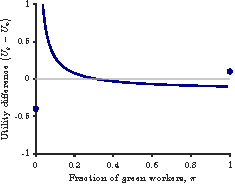
\includegraphics[width=0.5\textwidth]{figure1.pdf}
  \caption{Multiple Equilibria}
  \label{fig:psis}
  \medskip
  \footnotesize
  \textit{Notes:} The blue curve shows the utility advantage of green work relative to non-green work as the share of green workers increases. The horizontal zero line marks indifference; crossings and dots are equilibria.
\end{figure}

\subsection{Comparative Statics}\label{oneshot cs}

I conduct comparative statics in this static setting to show that each policy instrument can individually expand the green sector when the other instruments are held fixed. Consistent with the model’s mechanisms, Figure~\ref{fig:relative_static} shows that lowering the effective entry cost for workers (higher $s_g$ or lower $\kappa_g$) monotonically increases equilibrium green entry. Likewise, Figure~\ref{fig:effective_static} shows that raising the production-side subsidy $\tau_g$ increases green entry by improving vacancy profitability and, via free entry, market tightness. Taken together, the comparative statics establish that either margin, worker entry or firm vacancy creation, can scale the green sector on its own.


\begin{figure}[H]
  \centering

  \begin{subfigure}{0.5\textwidth}
    \centering
    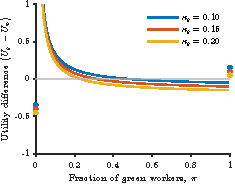
\includegraphics[width=\textwidth]{figure2a.pdf}
    \caption{Lower worker entry cost rauses green share.}
    \label{fig:relative_static}
  \end{subfigure}\hfill
  \begin{subfigure}{0.5\textwidth}
    \centering
    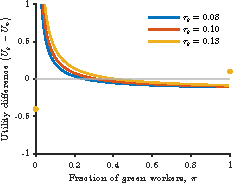
\includegraphics[width=\textwidth]{figure2b.pdf}
    \caption{Higher firm subsidy raises green share.}
    \label{fig:effective_static}
  \end{subfigure}

  \captionsetup{width=0.85\textwidth}
  \caption{Two policy levers to raise green employment.}
  \medskip
  \footnotesize
  \textit{Notes:} Axes are the same as in Figure~\ref{fig:psis}; Comparative statics are with respect to each policy margins holding other parameters fixed.
  \label{fig:comparative}
\end{figure}

\noindent Taken together, the static benchmark shows that either margin—worker entry support or firm production support—can, by itself, expand a sector with a positive externality. This motivates the dynamic analysis that follows, which designs policies to achieve that expansion \emph{most efficiently} by characterizing the scale, timing, and composition of support that minimize unemployment and fiscal outlays while improving welfare. The static setting also provides a clear framework for the underlying efficiency logic: it isolates the environmental externality that motivates policy-induced reallocation in the first place, clarifies its interaction with the standard search externality, and shows how alternative instruments can decentralize the planner’s allocation.


\subsection{Social Efficiency and Policy Implications}\label{sec:efficiency}

The decentralized equilibrium may be inefficient for two reasons:  
(i) standard search-and-matching externalities, and  
(ii) uninternalized environmental externalities from green job creation.  
I characterize efficiency using a social planner who internalizes both. 
% \footnote{All proofs and derivations are provided in~\ref{app:planner}.}
All proofs and derivations are provided in~\ref{app:planner}.


\subsubsection{Planner’s Problem Without Environmental Externalities}

If green jobs yield no external benefits ($\phi=0$), the planner maximizes total surplus:
\begin{equation}
\begin{split}
\max_{\{\pi,v_g,v_n\}} 
L(\pi,v_g,v_n)
=\; &\underbrace{\pi\,\frac{v_g}{\pi+v_g}(p-z)}_{\text{Green matches}}
+\;\underbrace{(1-\pi)\,\frac{v_n}{(1-\pi)+v_n}(p-z)}_{\text{Non-green matches}} \\
&\; - c(v_g+v_n) - \pi \kappa_g.
\end{split}
\label{eq:planner-obj}
\end{equation}


\begin{proposition}\label{prop:efficiency}
Without externalities ($\phi=0$), the planner’s solution is a corner: if $\kappa_g>0$, then $\pi^*=0$ and all workers enter the non-green sector. No interior allocation is efficient.
\end{proposition}

\textit{Proof in~\ref{app:planner-A}}.  

\noindent This result arises because the private cost of green entry $\kappa_g$ dominates any productivity gains, making the non-green allocation efficient.

\subsubsection{Planner’s Problem With Environmental Externalities}

When each green match generates an additional benefit $\phi>0$ accruing to society, the planner maximizes:
\begin{align}
\max_{\{\pi,v_g,v_n\}} 
L(\pi,v_g,v_n)
&=\; \underbrace{\pi\,\frac{v_g}{\pi+v_g}\bigl[(p-z)+\phi\bigr]}_{\text{Green matches with externality}}
+\;\underbrace{(1-\pi)\,\frac{v_n}{(1-\pi)+v_n}(p-z)}_{\text{Non-green matches}} \nonumber\\
&\quad - c(v_g+v_n) - \pi \kappa_g.
\label{eq:planner-obj-ext}
\end{align}

In the decentralized equilibrium, this externality is not internalized by workers or firms, leading to underinvestment in green employment.

\begin{proposition}\label{prop:full-efficiency}
With $\phi>0$, efficiency requires three alignment conditions:  
\begin{enumerate}
    \item Hosios condition: $\eta^{g*}=\frac{v_g^*}{\pi^*+v_g^*}=\eta^{n*}=\frac{v_n^*}{(1-\pi^*)+v_n^*}=\eta$, i.e. bargaining power equals the matching elasticity in both sectors.  
    \item Firm-side alignment: $\phi = \dfrac{\tau_g+\tau_n}{1-\eta}$.  
    \item Worker-side alignment: $\phi = \dfrac{\tau_g+\tau_n}{\eta(1-s_g)}$.  
\end{enumerate}
\end{proposition}

\textit{Proof in~\ref{app:planner-B}}.  

\noindent In addition to the standard Hosios condition, efficiency requires that policy instruments $(\tau,\tau_g,s_g)$ jointly align private and social returns for both firms and workers. Because these instruments are interdependent, not all combinations decentralize the planner’s allocation. Comparative statics in the one-shot model illustrate these policy channels.

\medskip

\noindent I now turn to the dynamic version of the model, which incorporates unemployment dynamics and policy financing over time.

\subsection{Dynamic Model: Extended DMP Framework}
\label{sec:dynamic-model}

Building on the static framework, the dynamic model introduces time and sectoral dynamics to analyze green labor market transitions more comprehensively. This extension permits a unified treatment of unemployment dynamics, funding requirements, and aggregate welfare, the central issues for policy design in the green transition.

\subsubsection{Physical Environment}
Time is discrete, $t=0,1,2,\dots$. Agents discount at rate $\beta\in(0,1)$. The labor force is normalized to 1. The economy features two segmented labor markets, green ($g$) and non-green ($n$). Existing matches are destroyed at rate $\lambda\in(0,1)$. The government provides a production subsidy $\tau_g$ to green firms financed by a tax $\tau_n$ on non-green firms. Workers entering the green sector incur a recurring entry cost $\kappa_g$, partially offset by a subsidy $s_g \geq 0$; entry into the non-green sector is costless.

\subsubsection{Matching Function}
Matching in each sector \(j \in \{g,n\}\) uses the same constant-returns (CRS) harmonic-mean technology as in the static benchmark:
\[
m_j(u_j,v_j)\;=\;\delta_j\,\frac{u_j v_j}{u_j+v_j},
\]
where \(u_j\) and \(v_j\) denote unemployed workers and vacancies, and \(\delta_j\) is sector-specific matching efficiency. The implied meeting probabilities are
\begin{equation}
\alpha_{wj}\;=\;\frac{m_j}{u_j}\;=\;\delta_j\,\frac{v_j}{u_j+v_j},\qquad
\alpha_{fj}\;=\;\frac{m_j}{v_j}\;=\;\delta_j\,\frac{u_j}{u_j+v_j},\qquad j\in\{g,n\}.
\label{matching prof}
\end{equation}

\subsubsection{Discussion of Modeling Choices and Empirical Relevance}
\label{section model discussion}
Before I move on to the full quantitative analysis, I want to discuss some modeling choices. \\
\\
\noindent\textbf{Definition of green jobs:}
Green jobs are defined following \citet{curtis2022green} as employment in renewable energy sectors (solar, wind, EVs), aligning with policy focus under the IRA and the fact that fossil fuel combustion accounts for roughly three-quarters of total U.S. greenhouse gas emissions \citep{epa2024inventory,eia2024sources}. This operational definition complements broader institutional notions \citep{ilo2018weso} and task-based classifications (O*NET; \citealp{vona2018greenskills,consoli2016skills,vona2019measures}) while capturing emerging occupations (e.g., solar installers).
\medskip

\noindent\textbf{Firm subsidies, $\tau_g$:}
The Inflation Reduction Act (IRA) provides substantial production and investment tax credits (\(\tau_g\)) to incentivize renewable energy deployment; in 2023 the full rate was about \$27.5/MWh, with additional domestic-content and energy-community bonuses available \citep{epa_ira_summary,irs_domestic_content}. This maps transparently into firms’ marginal revenues and fiscal cost. Evidence from labor-policy groups documents that, while these credits have accelerated deployment, workforce development remains a binding bottleneck \citep{linkedin2024stocktake,bga_nsc_2024,bluegreen_2024_shortages}. Hence I pair $\tau_g$ with a worker-side instrument in the design problem.

\medskip
\noindent\textbf{Worker entry costs:}
The parameter $\kappa_g$ represents the effective cost faced by a worker searching or transitioning into the green sector. In the model, it enters as a per-period flow cost borne by unemployed workers who choose to enter the green market. This reduced-form formulation captures a range of structural barriers observed in practice:
\begin{itemize}
  \item \textit{Training Costs:} Green jobs often demand new technical and managerial skills, requiring reskilling even in related occupations \citep{vona2018greenskills,consoli2016skills,bowen2018characterising}.
  \item \textit{Relocation Costs:} Green jobs are geographically dispersed, creating location mismatch that often requires moving from fossil-fuel hubs to renewable-resource regions \citep{lim2023location,greenspon2024matching,brookings2021uplift,vanatta2022siting}.
  \item \textit{Unionization and benefits:} Fossil-fuel and legacy utility occupations have historically higher union density and more comprehensive benefits than many emerging clean-energy occupations, which can deter transitions in the absence of labor standards \citep{muro2019clean,zabin2020highroad,zabin2021lessons}.
  \item \textit{Uncertainty and behavioral barriers:} Investment under uncertainty and real-option effects, together with behavioral frictions such as sunk-cost sensitivity and risk/time preferences in job search, further impede transitions \citep{dixit1994investment,arkes1985psychology,dellavigna2005jobsearch}.
\end{itemize}
Although the model remains agnostic about the precise composition of $\kappa_g$, it can be interpreted as the expected cost of remaining in the transition state. Figure~\ref{fig:green_supply_demand_gap}, from \citep{linkedin2024stocktake}, shows demand outpacing supply on an indexed basis, consistent with a supply-side constraint on worker entry. I therefore model $\kappa_g$ as the wedge that keeps potential movers from entering, and use $s_g$ to relax that constraint alongside firm-side incentives.

\medskip
\noindent\textbf{Policy design for $s_g$:}
In implementation, $s_g$ should be viewed as a package tailored to the dominant components of $\kappa_g$. A full structural decomposition of $\kappa_g$ is left for future work; here I note plausible mappings that respect the model’s timing (entry/search rather than post-hire):
\begin{itemize}[leftmargin=1.4em,itemsep=2pt]
\item \emph{Training/reskilling cost}: tuition waivers, training vouchers, certification grants.
\item \emph{Relocation/spatial cost}: relocation stipends, temporary housing or commuting subsidies, mobility grants to certified green regions.
\item \emph{Information/matching cost}: placement services with outcome-based payments, interview travel grants, fast-track credential recognition.
\item \emph{Benefits/union differential}: temporary wage insurance or portable benefits during transition (health coverage, retirement credits).
\end{itemize}
These instruments operate on the entry margin directly in contrast to wage or production credits that pay only once a match forms and are therefore the natural empirical counterparts to $s_g$ in the model.

\begin{figure}[H]
  \centering
  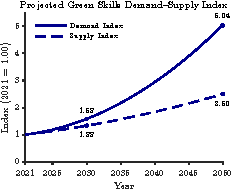
\includegraphics[width=0.5\linewidth]{figure3.pdf}
  \caption{Green Talent Demand and Supply (Indexed; Projections to 2050)}
  \medskip
  {\footnotesize
  \textit{Notes:} Figure~\ref{fig:green_supply_demand_gap} plots global indexes of green demand (solid) 
  and green talent supply (dashed). Both series are normalized to 1 in 2021; projections from 2025 onward 
  use median values and compound annual growth rates. By 2050, demand is $\approx$5.0 and supply  $\approx$2.5, 
  indicating a widening gap. 
  \textit{Source:} Author’s calculations adapted from \cite{linkedin2024stocktake}.}
  \label{fig:green_supply_demand_gap}
\end{figure}

\medskip
\noindent\textbf{Why focus on policy, and why now?}
Environmental externalities and near-approaching net-zero timelines imply that laissez-faire reallocation is inefficiently slow even with well-functioning markets. Historical restructurings show that unmanaged shifts can generate persistent local unemployment and scarring \citep{Oei2020}. The relevant question is therefore not \emph{whether} to intervene but \emph{how} to design instruments that meet a green employment target. This motivates the paper’s focus on policy design under two-sided coordination frictions.

\subsubsection{Analysis of the Model}

I derive equilibrium conditions linking policy instruments to Beveridge curves, value functions, and wages. This structure permits quantitative evaluation of green employment targets and the associated unemployment and fiscal paths.

\paragraph{Beveridge curves} Let $u$ denote the total unemployed workers who choose to enter either the green ($u_g$) or non-green ($u_n$) sector, where they may find a job and transition to employment ($e_g$ and $e_n$, respectively). Similarly, employed workers in both sectors face the possibility of job destruction at rate $\lambda$, which returns them to unemployment. The worker-flow diagram in Figure~\ref{figure model} implies steady-state relationships:
\begin{equation}
\alpha_{wg}u_g=\lambda e_g,\qquad \alpha_{wn}u_n=\lambda e_n,\qquad u_g+u_n+e_g+e_n=1. 
\label{eq bc}
\end{equation}
\begin{figure}[H]
\centering
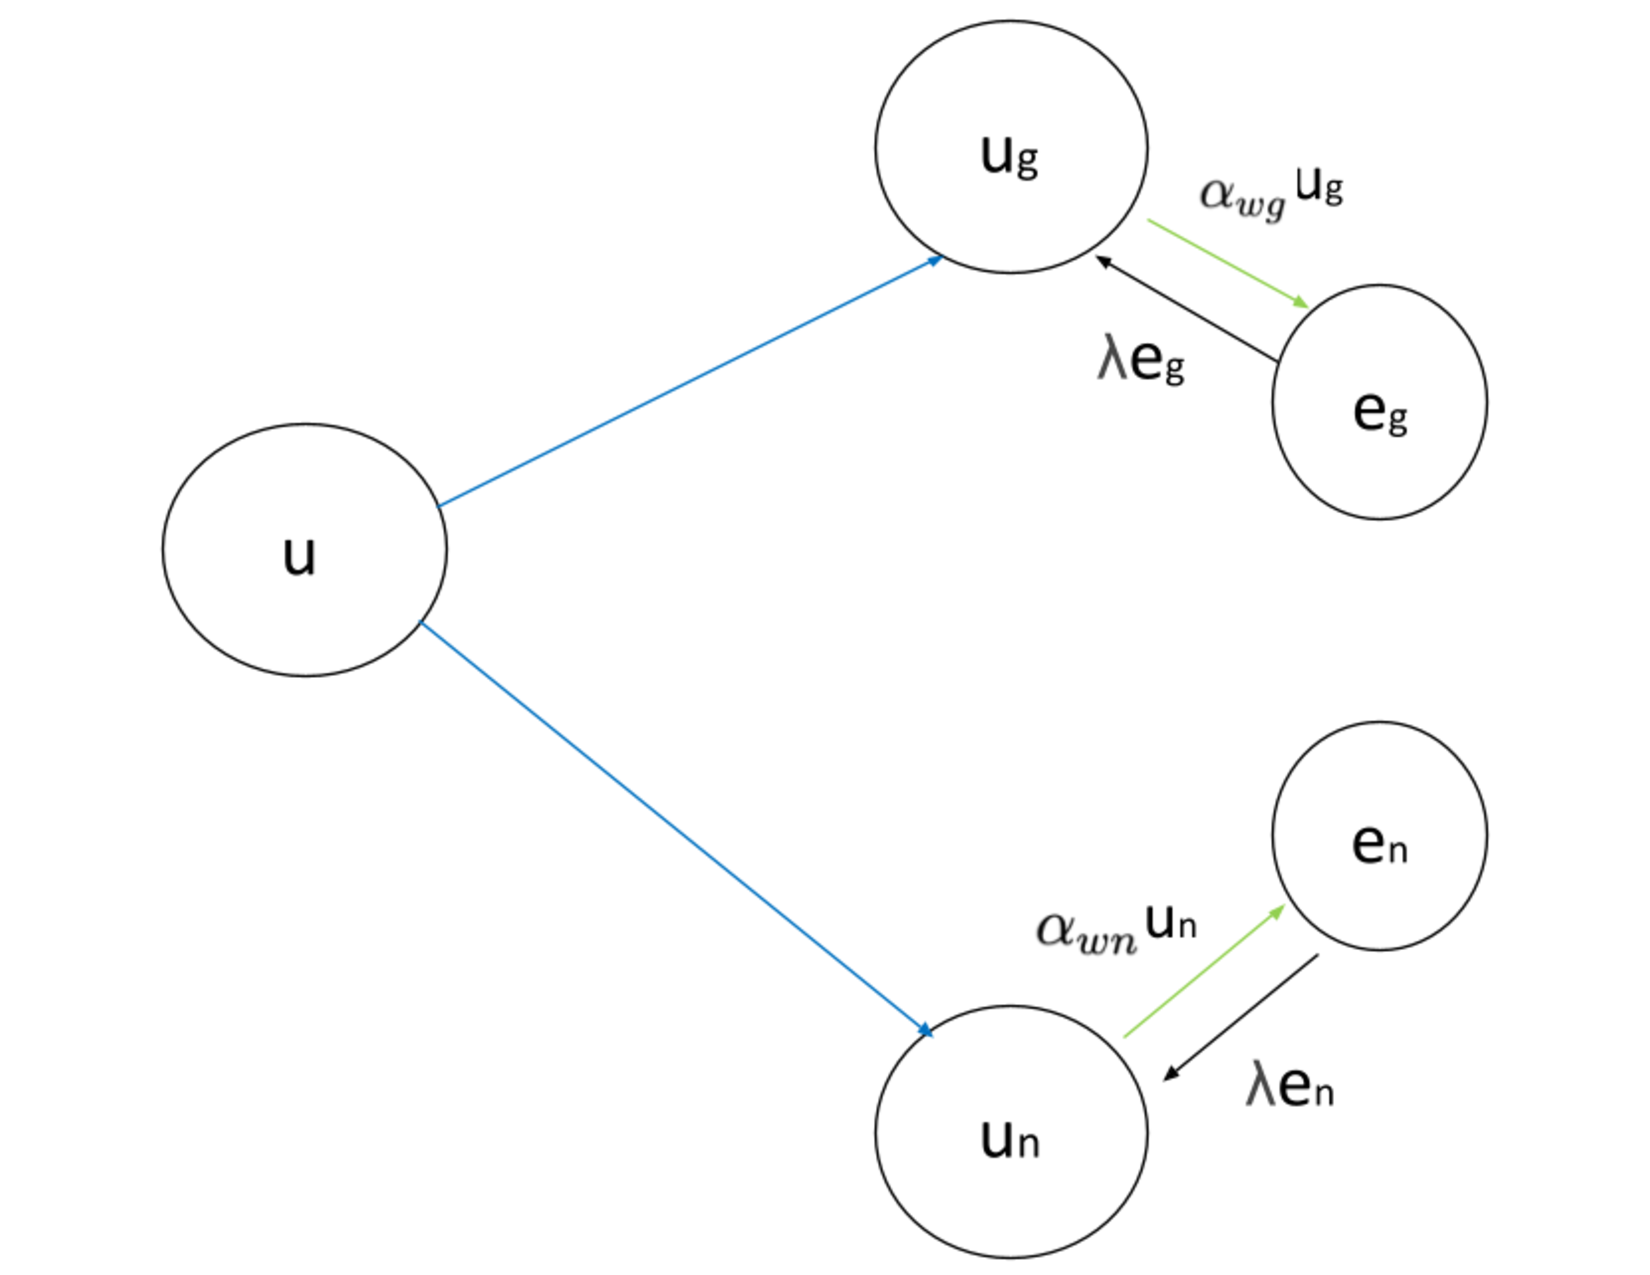
\includegraphics[width=0.5\linewidth]{figure4.pdf}
\vspace{-0.2cm}
\caption{Worker flows between unemployment and employment in both sectors.}
\label{figure model}
\end{figure}
\paragraph{Firms’ value functions and free entry} Firms choose between entering the green or non-green sectors based on expected profits, which is analogous to free entry in both sectors. Let \( V \) represent the value of a vacant firm, and \( V_g\) and \( V_n\) be the values of vacant jobs in the green and non-green sectors, respectively. Similarly, $J_g$ is the value of filled jobs in green sector and $J_n$ in the non-green sector respectively. Each value function is then: 


\begin{align}
V &= \max\{V_g, V_n\},
\label{eq:V_def} \\[4pt]
V_g &= -\,c \;+\; \beta\big[\alpha_{fg} J_g + (1-\alpha_{fg}) V\big],
\label{eq:vacant_value_g} \\[4pt]
V_n &= -\,c \;+\; \beta\big[\alpha_{fn} J_n + (1-\alpha_{fn}) V\big],
\label{eq:vacant_value_n} \\[4pt]
J_g &= (p+\tau_g) - w_g \;+\; \beta\big[\lambda V + (1-\lambda) J_g\big]\footnotemark,
\label{eq:filled_value_g} \\[4pt]
J_n &= p - \tau_n - w_n \;+\; \beta\big[(1-\lambda) J_n + \lambda V\big].
\label{eq:filled_value_n}
\end{align}

\footnotetext{Since I normalize productivity $p$ to 1 in the quantitative analysis, the green subsidy $\tau_g$ can be interpreted either as an additive transfer to firm revenue or equivalently as a per-unit output subsidy.} 

\noindent Free entry in both sectors implies $V_g=V_n=V=0$, yielding
\begin{align}
c &=\beta\alpha_{fg}J_g,\qquad c=\beta\alpha_{fn}J_n.
\label{eq free entry}
\end{align}
Imposing free entry to the value functions for filled firms also gives: 
\begin{equation}
J_g=(p+\tau_g)-w_g+\beta(1-\lambda)J_g,\qquad
J_n=p-w_n-\tau_n+\beta(1-\lambda)J_n.
\label{j}
\end{equation}

\paragraph{Workers’ value functions and optimal sector choice}
Following segmented-search models with stationary policies (see \citet{GeromichalosKospentaris2022Merit}), I first allow an unemployed worker to reconsider the sector if still unemployed, and then specialize to the stationary branch actually chosen. The Bellman system is
\begin{align}
U &= \max\{U_g,\,U_n\}, \label{eq:U_def}
\end{align}
with sector-specific unemployment values
\[
U_g = z - (\kappa_g - s_g) + \beta\!\left[\alpha_{wg}\, W_g + (1-\alpha_{wg})\, U\right],\]
\[
U_n = z + \beta\!\left[\alpha_{wn}\, W_n + (1-\alpha_{wn})\, U\right].
\]
In a stationary environment the sign of $U_g-U_n$ is constant, so \(U\) selects one branch and the unemployment recursion collapses to
\begin{align}
U_g &= z - (\kappa_g-s_g) \;+\; \beta\big[\alpha_{wg}\, W_g + (1-\alpha_{wg})\, U_g\big], \label{eq:unemployed_value_g} \\[4pt]
U_n &= z \;+\; \beta\big[\alpha_{wn}\, W_n + (1-\alpha_{wn})\, U_n\big]. \label{eq:unemployed_value_n}
\end{align}

Similarly, the Bellman system for employed workers is
\begin{align}
W_g &= w_g \;+\; \beta\big[(1-\lambda)\, W_g + \lambda\, U\big], \label{eq:employed_value_g} \\[4pt]
W_n &= w_n \;+\; \beta\big[(1-\lambda)\, W_n + \lambda\, U\big]. \label{eq:employed_value_n}
\end{align}

Solving for $U_g$ and $U_n$ yields
\[
U_g=\frac{[1-\beta(1-\lambda)]\big(z-(\kappa_g-s_g)\big)+\beta\,\alpha_{wg}\,w_g}{(1-\beta)\big(1-\beta(1-\alpha_{wg}-\lambda)\big)},
\]
\[
U_n=\frac{[1-\beta(1-\lambda)]\,z+\beta\,\alpha_{wn}\,w_n}{(1-\beta)\big(1-\beta(1-\alpha_{wn}-\lambda)\big)}.
\]

In equilibrium, workers are indifferent across sectors, $U_g = U_n$, which pins down the endogenous composition of search across $g$ and $n$:
\begin{equation}
\frac{[1-\beta(1-\lambda)]\big(z-(\kappa_g-s_g)\big) + \beta\, \alpha_{wg}\, w_g}{(1-\beta)\big(1-\beta(1-\alpha_{wg}-\lambda)\big)}
=
\frac{[1-\beta(1-\lambda)]\,z + \beta\, \alpha_{wn}\, w_n}{(1-\beta)\big(1-\beta(1-\alpha_{wn}-\lambda)\big)}.
\label{eq optimal entry}
\end{equation}

\subsubsection{Bargaining Problems}

\noindent \textbf{Non-green sector:} Let us start by describing the terms of trade in a meeting between a firm and an unemployed in the non-green sector. Solving the standard Nash bargaining problem leads to the following condition that must be satisfied:
\begin{equation}
(1-\eta)(W_n-U_n) = \eta J_n,
\end{equation}
This condition indicates that each party receives a share of the total surplus from the match, proportional to their bargaining power. (Recall that $\eta$ represents the worker’s bargaining power.) Substituting the value functions \( J_n \), \( U_n \), and \( W_n \) from above equations (12), (17), and (19) respectively, I can express the wage in the non-green sector as follows:
\begin{equation}
w_n=\frac{(1-\eta)z\,[1-\beta(1-\lambda)]+\eta(p-\tau_n)\,[1-\beta(1-\lambda-\alpha_{wn})]}{1-\beta(1-\lambda-\eta\alpha_{wn})}.
\label{eq wage nongreen}
\end{equation}
(See~\ref{app nongreen wage}.) The wage depends on tightness through $\alpha_{wn}$ and falls with the tax $\tau_n$.

\paragraph{Green sector}
Next, consider the bargaining problem between a firm and a worker in the green sector, where workers incur real costs to enter the sector, while firms receive government subsidies when they match with workers and produce. Again, I have:
\[
(1-\eta)\big(W_g-U_g\big)=\eta J_g,
\]
which yields
\begin{equation}
w_g=\frac{(1-\eta)\big(z-(\kappa_g-s_g)\big)\,[1-\beta(1-\lambda)]+\eta(1+\tau_g)p\,[1-\beta(1-\lambda-\alpha_{wg})]}{1-\beta(1-\lambda-\eta\alpha_{wg})}.
\label{eq wage green}
\end{equation}
(See~\ref{app green wage}.) The wage rises with firm- and worker-side support ($\tau_g$ and $s_g$) and declines with higher entry costs $\kappa_g$.

\subsubsection{Government Budget Constraint}
\label{gov}
Tax revenues from the non-green sector finance subsidies to green firms and workers:
\[
\underbrace{\tau_n \cdot \alpha_{fn} v_n}_{\text{Tax revenue from non-green firms}}
\;=\;
\underbrace{\tau_g \cdot \alpha_{fg} v_g}_{\text{Subsidies to green firms}}
\;+\;
\underbrace{s_g \cdot u_g}_{\text{Subsidies to green workers}}.
\]

\begin{equation}
\tau_n
=\frac{\tau_g\,\alpha_{fg}v_g+s_g\,u_g}{\alpha_{fn}v_n},
\label{gov budget}
\end{equation}
where $\alpha_{fj}$ are firm matching rates and $u_g,v_g,v_n$ denote the relevant stocks.

\subsubsection{Definition of Steady-State Equilibrium}
\label{definition equilibrium}
     A steady state equilibrium of the model consists of wages $(w_g, w_n)$ for workers in the green and non-green sectors, a green production subsidy $\tau_g$, a flat tax $\tau_n$ paid by non-green firms, measures of vacancies in both sectors $(v_g, v_n)$, and measures of employed and unemployed workers in the various states $(u_g, u_n, e_g, e_n)$. The subsidy and tax satisfy the government budget constraint (\ref{gov budget}). The remaining equilibrium variables satisfy two free entry conditions (\ref{eq free entry}), two wage curves ( \ref{eq wage nongreen}, \ref{eq wage green}), three Beveridge curves (\ref{eq bc}), and optimal entry condition (\ref{eq optimal entry}),  after one replaces the various $\alpha$'s with the respective matching probabilities given in (\ref{matching prof}). 

\section{Calibration}

I calibrate the benchmark model to the U.S. economy in 2022, focusing on labor market dynamics in the green transition. One model period corresponds to one calendar month. Parameters with direct empirical counterparts are set exogenously. The discount factor is $\beta=0.9959$, consistent with a 5\% annual interest rate. Worker productivity $p$ is normalized to 1. Following \citet{shimer2005cyclical}, workers’ bargaining power is set to $\eta=0.72$, and the non-employment benefit to $z=0.4p$ (40\% of average productivity).  

Several calibration targets discipline the model. First, I target a 2\% wage premium for green workers relative to non-green workers, based on IMF staff estimates \citep{imf2022}.\footnote{Other studies find larger premiums, e.g., about 4\% in \citet{voxeu2023} and up to 20\% in \citet{curtis2022green}, but I adopt the conservative estimate.} Second, the green employment share is set at 2\% of the total U.S. workforce, consistent with 2022 estimates from the Energy Information Administration \citep{eia2024} and calculation of employment share in the renewable sector\footnote{In 2022, there were 3.3 million renewable energy jobs \citep{E2CleanJobs2023} and 212.4 million total jobs \citep{BEA_SAEMP25N_2024}, resulting in $e_g/e \approx 2\%$.}. Third, the hiring likelihood ratio for workers with green skills relative to others is set to 29\%, as reported by LinkedIn’s \emph{Green Skills Report} \citep{LinkedInGreenSkillsReport}. Fourth, overall labor market tightness, measured as the ratio of vacancies to unemployed workers, is set to 1.868, using BLS JOLTS job openings and CPS unemployment, retrieved via FRED \citep{BLS_JTSJOL,BLS_UNEMPLOY}. Finally, the unemployment rate is targeted at 3.5\%, matching BLS data for 2023 \citep{bls2023}.  

I also incorporate the scale of green subsidies under the Inflation Reduction Act (IRA). Production and investment tax credits range from \$5/MWh to \$32/MWh depending on eligibility \citep{bushnell2024modeling}. With 0.91 billion MWh of renewable generation in 2022 \citep{doe2023} and GDP of \$25.44 trillion \citep{worldbank2022}, these subsidies correspond to 0.018--0.114\% of GDP. I set the benchmark subsidy rate at 0.10\% of GDP for three reasons: (i) effective rates often sit near the upper tier once bonus provisions (prevailing wage, domestic content, energy communities) are met \citep{bushnell2024modeling}; (ii) using 2022 generation is conservative given the near-term pipeline, so the GDP share of credits can be closer to the top of the interval; and (iii) the higher benchmark provides a fiscal stress test. Qualitative rankings are unchanged across the full 0.018--0.114\% range.

\noindent The model matches the targeted moments closely, as shown in Table~\ref{tab:targets}.  

\begin{table}[H]
\centering
\begin{tabular}{lcc}
\hline
\textbf{Moment} & \textbf{Model} & \textbf{Target} \\
\hline
Wage premium (green/non-green) & 1.02 & 1.02 \\
Employment share (green)       & 0.0195 & 0.0195 \\
Hiring likelihood ratio         & 1.29 & 1.29 \\
Labor market tightness          & 1.868 & 1.868 \\
Unemployment rate               & 3.5\% & 3.5\% \\
\hline
\end{tabular}
\caption{Model performance in matching calibration targets.}
\label{tab:targets}
\end{table}

\noindent The internally calibrated parameters needed to match these moments are reported in Table~\ref{param}.  

\begin{table}[H]
\centering
\begin{tabular}{lcc}
\hline
\textbf{Parameter} & \textbf{Description} & \textbf{Value} \\
\hline
$c$        & Vacancy creation cost            & 0.1223 \\
$\lambda$  & Separation rate                  & 0.0192 \\
$\delta_g$ & Matching efficiency (green)      & 0.8476 \\
$\delta_n$ & Matching efficiency (non-green)  & 0.8165 \\
$\kappa_g$ & Worker entry cost (green)        & 0.7146 \\
\hline
\end{tabular}
\caption{Internally calibrated parameters.}
\label{param}
\end{table}

\noindent \textit{Identification:} The separation rate $\lambda$ is calibrated to match the steady-state unemployment rate $(3.5\%)$, the vacancy cost $c$ to aggregate tightness $(\theta=1.87)$, the worker entry cost $\kappa_g$ to the green employment share $(2\%)$, and the relative matching efficiency parameters $(\delta_g, \delta_n)$ to replicate the hiring-likelihood ratio $(1.29)$ and the green wage premium $(1.8\%)$. 

\medskip 

\noindent \textbf{Validation of Non-Targeted Moments:}\footnote{Official series (CPS, JOLT) do not classify jobs as “green” vs. “non-green,” so sector-specific tightness and matching rates are not directly observable. I therefore benchmark model-implied ratios against established external indicators.}

\noindent \emph{Tightness asymmetry:} With the green sector at 1.95\% of employment, the non-green market effectively tracks the aggregate economy. Consistent with this, the targeted aggregate tightness ($\theta=1.868$) aligns with the model’s non-green tightness ($\theta_n=1.83$). The model predicts a tightness wedge $\theta_g/\theta_n=2.24$. As a proxy, clean-energy job growth of 4.9\% versus 2.0\% for the overall U.S. economy \citep{DOE_USEER_2024} implies a ratio of $2.45$. While growth rates are proxy statistics for tightness, the magnitude is comparable (2.24 vs.\ 2.45).

\noindent \emph{Vacancy-filling difficulty:} The model implies that green vacancies are harder to fill, with $q_g/q_n=0.58$ (about 42\% lower fill probability). External skill-demand indicators point to a comparable supply-demand mismatch identified in \citet{linkedin2024stocktake} (see Figure~\ref{fig:green_supply_demand_gap}). That report projects a green talent supply-to-demand ratio of: $2.5/5.0 = 0.50$, consistent with persistent excess demand for green skills.

\noindent Taken together, these checks support the model’s core asymmetry of tighter green markets and more difficult vacancy filling within reasonable empirical bounds given current data coverage.

\medskip 

\noindent This calibration anchors the model to key features of the U.S. labor market and provides a benchmark for policy experiments. With the model successfully reproducing the wage premium, employment shares, hiring patterns, tightness, and unemployment rate, I am equipped to address the central policy question: \emph{Which mix of worker-side and firm-side interventions can raise green employment from 2\% to 14\% of the labor force by 2030, as projected by \citet{workingnation2024greenjobs}, while minimizing unemployment, costs and welfare distortions?}

\section{Quantitative Analysis}

The U.S. aims to raise the share of green employment from 2\% to 14\% of total jobs by 2030, implying nearly 24 million green jobs \citep{workingnation2024greenjobs}. Using the calibrated model, I evaluate the policy levers needed to achieve this target, focusing on two margins: (i) lowering worker entry costs into the green sector ($\kappa_g$, via subsidies $s_g$) and (ii) raising production subsidies for green firms ($\tau_g$). The analysis proceeds in three steps: Section~\ref{sec:reaching_target} shows that multiple instruments can reach the 14\% target; Sections~\ref{sec:unemployment_welfare} and \ref{sec:welfare_sensitivity} compare efficiency across unemployment, fiscal cost, and welfare; and Section~\ref{sec:transition_dynamics} characterizes the optimal dynamic policy along the transition path. Consistent with the static comparative statics (Figures~\ref{fig:relative_static} and \ref{fig:effective_static}), the dynamic analogue in Figures~\ref{fig:relative}--\ref{fig:effective} shows that each instrument, in isolation, can expand the green sector to the target when the other is held at baseline.


\begin{figure}[H]
  \centering
  \begin{subfigure}[b]{0.49\textwidth}
    \centering
    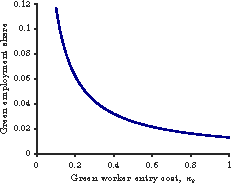
\includegraphics[width=\textwidth]{figure5a.pdf}
    \subcaption{Lower entry costs raise green jobs share.}
    \label{fig:relative}
  \end{subfigure}\hfill
  \begin{subfigure}[b]{0.49\textwidth}
    \centering
    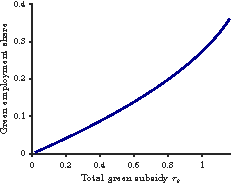
\includegraphics[width=\textwidth]{figure5b.pdf}
    \subcaption{Higher firm subsidies raise green jobs share.}
    \label{fig:effective}
  \end{subfigure}
  \caption{Dynamic model: two policy instruments to increase green employment.}
   \medskip
  \footnotesize
  \textit{Notes:} Panels show dynamic comparative statics holding other parameters fixed. Lower worker entry costs or higher firm subsidies increase the share of green jobs.
  \label{fig:dynamic_two_instruments}
\end{figure}


\subsection{Reaching the Green Employment Target}\label{sec:reaching_target}

The first goal of any policy design is simply to hit the target: expand the green sector to the required employment share. Table~\ref{table:green_employment_comparison} summarizes policy mixes that reach the 14\% target. Although all strategies succeed in principle, they differ markedly in composition and cost.

\begin{table}[htbp]
\centering
\caption{Alternative Policy Mixes Achieving 14\% Green Employment}
\begin{adjustbox}{max width=\textwidth}
\begin{tabular}{l *{4}{>{\raggedleft\arraybackslash}p{2.5cm}}}
\toprule
\textbf{Policy configuration} &
\textbf{Worker subsidy} & 
\textbf{Firm subsidy} & 
\textbf{Total subsidy} & 
\textbf{Green employment} \\
 & \textit{(\% of GDP)} & \textit{(\% of GDP)} & \textit{(\% of GDP)} & \textit{(\%)} \\
\midrule
Dual intervention & 0.48 & 0.07 & 0.55& 14.0 \\
Worker-only policy & 0.60 & 0.00 & 0.60 & 14.0 \\
Firm-only policy & 0.00 & 0.58 & 0.58 & 14.0 \\
\midrule
Baseline (2022) & 0.00 & 0.00 & 0.00 & 2.0 \\
\bottomrule
\end{tabular}
\end{adjustbox}
\begin{flushleft}
\footnotesize\textit{Note:}  
All policy configurations reach an equilibrium green employment share of 14\%, starting from a 2\% baseline.  
\end{flushleft}
\label{table:green_employment_comparison}
\end{table}

The baseline economy features only 2\% of total employment in the green sector.  
All three policy paths can reach the 14\% target, but they differ in the composition of fiscal support.  
The combined (dual) strategy achieves the target with the smallest total subsidy burden, indicating complementarity where each instrument makes the other more effective.

\subsection{Unemployment, Fiscal Cost, and Welfare Effects}\label{sec:unemployment_welfare}

Having established that multiple policy mixes can reach the 14\% green employment target, I now ask which mix is \emph{most efficient} once unemployment, fiscal cost, and welfare are taken into account. Since the policy rationale is to internalize an environmental externality, the welfare metric incorporates a positive green-job externality. I calibrate this externality $\phi$ to deliver a 2\% consumption-equivalent variation (CEV) gain at the target—consistent with the climate-macro literature that views the costs of inaction as large and justifying significant intervention (e.g., \citealp{Stern2008}). Section~\ref{sec:welfare_sensitivity} reports extensive sensitivity; the ranking of policies is robust across a wide range of $\phi$.

Table~\ref{table:welfare_funding} compares the outcomes, conditional on attaining 14\%, along unemployment, fiscal cost (as \% of GDP), and welfare (CEV relative to baseline). The \emph{dual} policy dominates: it achieves the highest welfare, the lowest unemployment, and the smallest fiscal outlay.

\begin{table}[htbp]
\centering
\caption{Policy Trade-offs: Unemployment, Fiscal Cost, and Welfare}
\label{table:welfare_funding}
\begin{adjustbox}{max width=\textwidth}
\begin{tabular}{l *{3}{>{\raggedleft\arraybackslash}p{4cm}}}
\toprule
\textbf{Policy configuration} &
\textbf{Unemployment} &
\textbf{Fiscal cost} &
\textbf{Welfare (CEV)}\\
& \textit{(\%)} & \textit{(\% of GDP)} & \textit{(\% vs.\ baseline)} \\
\midrule
\textbf{Dual intervention} & \textbf{4.77} & \textbf{0.55} & \textbf{1.12} \\
Worker-only policy & 5.16 & 0.60 & 0.83 \\
Firm-only policy & 4.79 & 0.58 & 0.89 \\
\midrule
Baseline (2022) & 3.50 & 0.00 & 0.00 \\
\bottomrule
\end{tabular}
\end{adjustbox}

\vspace{0.25em}
\footnotesize\textit{Notes:} Unemployment (\%), fiscal cost (\% of GDP), and welfare (CEV vs.\ baseline). The CEV calculation includes a calibrated green-job externality of $\phi=0.142$ corresponding to the 2\% CEV benchmark (see Section~\ref{sec:welfare_sensitivity}). Baseline (2022) CEV is normalized to zero (welfare level 0.9701).
\normalsize
\end{table}

\noindent Dual policy dominates on all three margins simultaneously; it is both cheaper (lower fiscal cost) and more effective (lower unemployment, higher welfare), making it the unambiguous policy recommendation. Quantitatively, relative to a worker-only subsidy, the dual policy raises welfare by 0.29 pp (29 bps) in CEV terms, reduces fiscal cost by 0.05 pp (5 bps) of GDP, and lowers unemployment by 0.39 pp (39 bps). Relative to a firm-only policy, welfare is higher by 0.23 pp (23 bps), fiscal cost is lower by 0.03 pp (3 bps), and unemployment is lower by 0.02 pp (2 bps). The next section examines how these conclusions vary with the magnitude of the externality. 


\subsection{Welfare Sensitivity to Green Externalities}
\label{sec:welfare_sensitivity}

To understand the robustness of my results, I now explore the sensitivity of welfare to the externality parameter, $\phi$. While my main results in Table~\ref{table:welfare_funding} assume $\phi = 0.142$ (the value required to generate a 2\% CEV gain), this section analyzes the full range of welfare outcomes. To do so, I incorporate a positive externality from green employment into the welfare function. The standard DMP welfare is
\[
W_0 \;=\; p(e_g+e_n) \;+\; (z-\kappa_g)u_g \;+\; z u_n \;-\; c(v_n+v_g),
\]
and adding a per-job externality $\phi$ (the environmental benefit per green job) gives
\[
W_\phi \;=\; p(e_g+e_n) \;+\; (z-\kappa_g)u_g \;+\; z u_n \;-\; c(v_n+v_g) \;+\; \phi\, e_g.
\]

\subsubsection{Threshold Analysis}

The welfare effects of policy depend critically on \(\phi\), the green-sector externality. Figure~\ref{fig:externality_plot} plots welfare relative to baseline, \(\Delta W(\phi)=W_\phi-W_0\), against \(\phi\). Under the dual policy, welfare equals the baseline at the threshold \(\phi^\star\) (i.e., \(W_\phi=W_0\)). For \(\phi<\phi^\star\), welfare is below baseline; at \(\phi=\phi^\star\), it is equal to baseline; and for \(\phi>\phi^\star\) (with \(\phi^\star\approx 0.062\)), welfare is above baseline. Hence only a modest externality is needed for the green reallocation to be welfare-improving.

\begin{figure}[H]
\centering
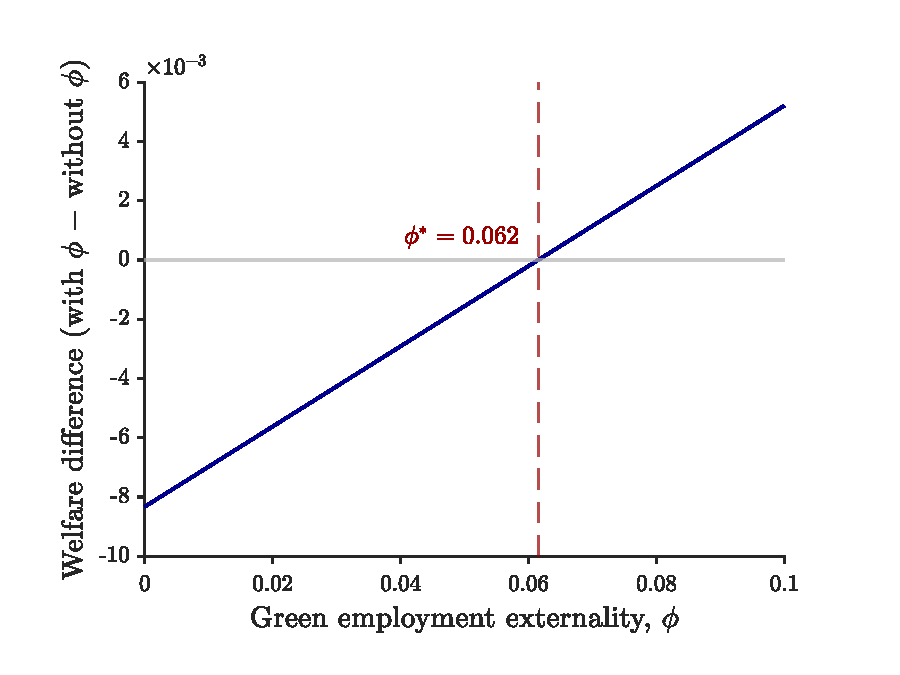
\includegraphics[width=0.65\linewidth]{figure6.pdf}
\caption{Welfare gains as a function of the externality parameter $\phi$ ($\phi^\star \approx 0.062$).}
  \medskip
  \footnotesize
  \textit{Notes:} Blue line: welfare with the externality minus the baseline. The zero line marks equal welfare. The dashed line shows the threshold $\phi^\star\!\approx\!0.062$; welfare is positive for $\phi>\phi^\star$ and negative for $\phi<\phi^\star$.

\label{fig:externality_plot}
\end{figure}

\subsubsection{Consumption-Equivalent Interpretation}

To make the magnitude of $\phi^\star$ interpretable, I translate it into a \emph{consumption-equivalent} change, i.e., the percent increase in consumption that delivers the same welfare gain.\footnote{CEV is computed from the ratio $W_{\phi^\star}/W_0$ under the maintained linear-utility (CRRA $\sigma=0$) index used throughout.} In the calibrated economy, the threshold is $\phi^\star \approx 0.0615$ per green job, at which welfare rises from $W_0=0.961$ to $W_{\phi^\star}=0.970$ while the target share remains $L_g=14\%$. The implied consumption-equivalent gain is CEV $=0.866\%$ relative to baseline. Thus, only a modest externality on the order of a $0.87\%$ consumption-equivalent improvement is sufficient for the transition to become welfare-improving.

\subsection{Transition to a 14\% Green Share}\label{sec:transition_dynamics}
I implement the transition as a sequence of policy–induced steady states that hit intermediate adoption targets. For each target green employment share \(L_g \in \{2\%,4\%,\ldots,14\%\}\), I solve for the welfare–maximizing mix of worker-entry support \((s_g)\) and firm-side production subsidies \((\tau_g)\) subject to equilibrium conditions and a balanced budget. The next target uses the previous solution as a warm start, generating a controlled path of \((s_g,\tau_g)\), allocations, and prices indexed by the achieved \(L_g\). For each \(L_g\), I record unemployment, total funding as a share of GDP, and its worker/firm decomposition, and I track green tightness, the job-finding rate, and the vacancy-filling rate along the path.\footnote{With matching \(m_g=\delta_g\,u_g v_g/(u_g+v_g)\) and green tightness \(\theta_g\equiv v_g/u_g\), the rates are \(f(\theta_g)\equiv m_g/u_g=\delta_g\,\theta_g/(1+\theta_g)\) and \(q(\theta_g)\equiv m_g/v_g=\delta_g/(1+\theta_g)\). Hence \(f'(\theta_g)=\delta_g/(1+\theta_g)^2>0\) and \(q'(\theta_g)=-\delta_g/(1+\theta_g)^2<0\). In the figures, “pathwise elasticities’’ are computed as finite differences of \(f(\theta_g)\) and \(q(\theta_g)\) with respect to \(\theta_g\) along the sequence of steady states and serve as diagnostics for which margin (entry vs.\ vacancies) is locally more responsive.}

This transition study is deliberately not a full perfect-foresight transition. Instead, it is designed to mirror how climate policies are set and revised in practice. Under the Paris framework, countries submit Nationally Determined Contributions on a fixed cycle and are required to demonstrate a progression in ambition; likewise, major decarbonization roadmaps (e.g., the IEA’s \emph{Net Zero by 2050}) translate long-run goals into dated intermediate milestones rather than a single continuous optimal path.\footnote{See UNFCCC, \emph{Paris Agreement} 2015 (five-year cycle; successive NDCs must ``progress''); and IEA, \emph{Net Zero by 2050} (and 2023 update) for milestone-based planning.} In this institutional setting, the relevant policy objects are the least-cost instrument mix and associated fiscal burden at each interim target, not the solution to a fully forward-looking optimal control problem. A sequence of policy-induced steady states therefore delivers exactly the quantities that are observed and monitored in practice. 

Figure~\ref{fig:transition_decomp} shows the required fiscal outlays along the welfare–maximizing path are modest and \emph{hump–shaped} in the achieved green share \(L_g\). Total funding rises as the economy moves from low adoption toward intermediate targets, peaks in the middle of the transition, and gradually declines as \(L_g\) approaches 14\%. The composition of funding rotates with scale: worker–side support dominates at the beginning and end of the path, while firm–side production subsidies account for a larger share at intermediate targets.

\begin{figure}[H]
  \centering
  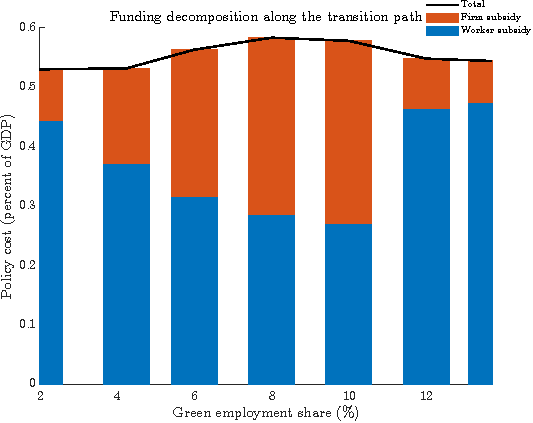
\includegraphics[width=0.65\linewidth]{figure7.pdf}
  \caption{Funding decomposition along the transition path}
  \label{fig:transition_decomp}
  \medskip
  \footnotesize
  \textit{Notes:} Bars split total funding into worker and firm components; the line overlays total funding relative to GDP. Figures are computed along the welfare-maximizing transition to 14\%.
\end{figure}

The hump and the rotation reflect how green labor–market tightness \((\theta_g)\) moves the marginal matching cost between the two sides of the market. Early in the transition, vacancies outpace entrants, so subsidies that lower the entry cost for workers are relatively powerful and inexpensive. At intermediate \(L_g\), tightness is high: job–finding flattens and vacancy–filling is slow, making both margins locally inelastic and pushing up the total cost of creating additional matches, hence the hump. As the target is approached, tightness eases and the marginal cost falls, leading funding requirements to taper and the mix to tilt back toward worker support. The full accounting of the green labor market dynamics, including tightness, the job–finding and vacancy–filling schedules, and the pathwise elasticities used as diagnostics, are provided in Appendix \ref{sec:appendix_transition} (see, e.g., Figures \ref{fig:app_transition_tightness_rates} and \ref{fig:app_transition_derivatives}).

\paragraph{Transition policy insights} Policy design and timing are both critical. While dual-sided support (targeting both workers and firms) is more efficient than one-sided policies for a given target $L_g$, the optimal mix of instruments is state-contingent. Specifically, the design should depend on which margin between unemployment (the worker-side) or vacancies (the firm-side) is the binding constraint on matching. For instance, the policy should prioritize worker support when the pool of unemployed entrants is the bottleneck, and shift toward firm subsidies when the lower vacancies is the key hindrance. Recognizing this state-contingency allows for a policy mix that remains cost-effective throughout the transition by always targeting the margin that binds most.

\section{Economic Insights}
Reallocation in this environment is shaped by two distinct externalities that interact to stall the transition. The first is the standard environmental externality that motivates expanding the green sector: decarbonization generates social benefits not captured in private decisions. The second is a coordination or matching externality endemic to search frictions but often overlooked in the climate-policy literature: workers' entry raises the value of firms' vacancies, and firms' vacancy creation raises the return to workers' entry. Because neither side internalizes the benefit it creates for the other, each under-invests even when the environmental case for expansion is clear. A dual policy that lowers worker entry costs and supports vacancy creation realigns private and social returns on both margins, restores complementarity, and raises matches per dollar of public spending under a balanced budget. These insights extend beyond decarbonization to any large-scale sectoral expansion where coordination failures between workers and firms impede reallocation, including advanced manufacturing scale-ups, digital adoption, pandemic preparedness, or post-trade-shock realignment.


\paragraph{Insight 1: Dual beats single on the margins that matter}
Worker-only or firm-only designs can raise the green share, but they leave the other side as the bottleneck, producing avoidable unemployment (idle search meets empty vacancies, or vice versa) and higher fiscal outlays per match. A coordinated, two-sided policy breaks the coordination friction by thickening the applicant pool and raising vacancy profitability at the same time. In the benchmark, the same 14\% target is achieved with materially lower unemployment and lower cumulative spending than the best one-sided alternative. This dominance is because the outcomes depend on complementary participation, so using both instruments outperforms subsidizing one side alone. Critically, this result departs from frictionless, neoclassical models where labor reallocates instantaneously and which side of the market the government supports is irrelevant; a lump-sum transfer to workers or an equivalent subsidy to firms would deliver identical outcomes at identical cost. Here, search frictions break that equivalence. Since matching requires time, coordination, and complementary investment by both sides, subsidizing workers alone leaves vacancies unfilled, while subsidizing firms alone leaves the worker pipeline thin.

\paragraph{Insight 2: State-contingent mix along the path}
Optimal policy targets the binding margin and rotates as tightness changes along the 2\% to 14\% path. Early, entry is scarce: the pool of potential movers is large and firms can absorb them, so tilting to worker support yields many matches per dollar; firm support is secondary. Midway, the market is tight and filling constraints bind: both margins are locally less responsive, total support peaks, and firm-side subsidies are especially effective. Late, vacancies fill more easily but the remaining pool of movers is thin: the constraint swings back to new entry, so the mix tilts again to worker support. The rule is simple: target the binding margin; rotate worker–firm–worker as the market evolves.

\paragraph{Insight 3: Welfare requires modest external benefits relative to reallocation costs}
Welfare reflects a trade-off between private reallocation costs and non-internalized external benefits. Expressed in consumption-equivalent terms, the transition is welfare-improving whenever the external benefit per additional match in the target sector exceeds the consumption-equivalent cost of creating that match. In the benchmark decarbonization application, a benefit on the order of a 0.87\% permanent consumption gain suffices. While the exact threshold is model-specific and depends on the magnitude of the externality, the principle of benefit greater than cost is general and applies to any sectoral expansion justified by non-internalized social returns. Importantly, this welfare criterion accounts for both externalities: the environmental benefit that justifies the expansion and the coordination externality that raises the fiscal and unemployment cost of achieving it. The framework thus provides a transparent welfare criterion applicable across mission-scale reallocations.

\section{Conclusion}

Green transition is not merely a technological challenge, it is fundamentally a reallocation problem constrained by labor-market frictions. This paper demonstrates that climate policy design must account for coordination failures between workers and firms, failures that compound the environmental externality and can stall decarbonization even when the social case for action is clear. I develop a two-sector search-and-matching framework calibrated to a U.S. transition from 2\% to 14\% green employment by 2030, quantifying policy design along three margins: unemployment costs, fiscal outlays, and aggregate welfare.

Three results emerge. First, which side of the market the government supports matters as much as the size of the support. Search frictions break the policy-irrelevance result standard in frictionless climate-macro models. A coordinated dual policy supporting worker entry \emph{and} firm production reaches the 14\% target with 39 basis points lower unemployment, 5 basis points of GDP lower fiscal cost, and 23 basis points higher welfare than the best single-instrument alternative. Second, optimal policy is state-contingent: total support is hump-shaped along the path, and its composition rotates: worker support dominates early and late, firm support mid-path when vacancy constraints bind. Third, the welfare threshold is modest: coordinated policy improves welfare when environmental benefits exceed 0.87\% of aggregate consumption, well within standard climate-damage estimates. Critically, the welfare criterion accounts for both externalities, environmental benefits and coordination frictions.

The lesson for climate policy is clear: labor reallocation policy is essential to climate policy. Decarbonization strategies relying solely on technology subsidies and carbon pricing will miss efficiency gains, hitting targets at 5–39 basis points higher cost in fiscal outlays and unemployment, the twin barriers to political feasibility.  This coordination problem extends beyond climate to any large-scale sectoral reallocation where workers and firms must move simultaneously.

% Add vertical space and a horizontal line
% \vspace{5cm} % Adjust the spacing as needed
% \noindent\rule{\textwidth}{0.4pt} % Creates a horizontal line across the page

% Add the additional content
% \noindent During the preparation of this work, the author used ChatGPT solely to format the LaTeX code and to edit the final content for clarity and presentation. After utilizing this tool, the author thoroughly reviewed and modified the content as necessary and takes full responsibility for the accuracy and integrity of the publication.

\newpage

\bibliographystyle{elsarticle-num-names}
\bibliography{main} 

\newpage

\appendix
% format the equation environment
\renewcommand{\theequation}{A.\arabic{equation}}

% reset the counter
\setcounter{equation}{0}

\section{One-shot DMP Model} \label{one-shot}

This section provides the detailed derivations for the static (one-period) benchmark version of the model, which is useful to illustrate the role of coordination frictions and the operation of policy instruments in segmented labor markets.  

\subsection{Bargaining}

\textbf{Green Sector:} In the green sector, wages are determined via Nash bargaining between firms and workers. The problem is
\begin{eqnarray*}
&& \max_{w_g} (w_g - z)^\eta \,(p + \tau_g - w_g)^{1-\eta}, \\
&& \implies \frac{\eta}{w_g - z} = \frac{1-\eta}{p + \tau_g - w_g}, \\
&& \therefore \; w_g = \eta (p + \tau_g) + (1-\eta) z.
\end{eqnarray*}
The bargained wage in the green sector is increasing in productivity \(p\) and the production subsidy \(\tau_g\), while the fallback option \(z\) provides the lower bound.

\medskip

\textbf{Non-Green Sector:} In the non-green sector, the structure of the bargaining problem is analogous, except that firms pay a per-unit tax \(\tau_n\):
\begin{eqnarray*}
&& \max_{w_n} (w_n - z)^\eta \,(p - \tau_n - w_n)^{1-\eta}, \\
&& \implies \frac{\eta}{w_n - z} = \frac{1-\eta}{p - \tau_n - w_n}, \\
&& \therefore \; w_n = \eta (p - \tau_n) + (1-\eta) z.
\end{eqnarray*}
Relative to the green sector, non-green wages are depressed by the tax burden \(\tau_n\).  

\subsection{Interior Equilibrium with Both Sectors Operating}

When both sectors are active, the equilibrium variables are \(\{\pi,v_g,v_n,w_g,w_n\}\), where \(\pi\) is the share of (initially unemployed) workers who \emph{enter the green market}. The conditions are:
\begin{eqnarray*}
&& c = \frac{\pi}{\pi+v_g}\big(p + \tau_g - w_g\big), \\
&& c = \frac{1-\pi}{1-\pi+v_n}\big(p - \tau_n - w_n\big), \\
&& w_g = \eta (p + \tau_g) + (1-\eta)z, \\
&& w_n = \eta (p - \tau_n) + (1-\eta)z, \\
&& \tau_n \,\frac{(1-\pi)}{(1-\pi)+v_n} v_n
= \tau_g \,\frac{\pi}{\pi+v_g} v_g \;+\; s_g \,\pi, \\
&& \pi = \begin{cases} 
0 & \text{if } G < N, \\
\in (0,1) & \text{if } G = N, \\
1 & \text{if } G > N,
\end{cases}
\end{eqnarray*}
where the expected utilities of workers (before matching) are
\[G \;=\; -(\kappa_g - s_g) \;+\; \frac{v_g}{\pi+v_g} \, w_g \;+\; \Big(1-\frac{v_g}{\pi+v_g}\Big) z,\]
\[
N \;=\; \frac{v_n}{1-\pi+v_n} \, w_n \;+\; \Big(1-\frac{v_n}{1-\pi+v_n}\Big) z.
\]
\emph{Notes:} (i) The government budget uses \emph{matches} as the base for firm-side flows and \emph{entrants} as the base for worker-side transfers. Since the unit mass of workers is initially unemployed and entry occurs \emph{before} matching, the mass receiving the level subsidy is \(\pi\). (ii) Throughout, \(s_g\) is a \emph{level} (per-period) subsidy; the effective worker cost is \(\kappa_g-s_g\).

\subsection{Corner Equilibria}

The economy can also settle in corner solutions.

\subsubsection{Case \(\pi=0\): Non-Green Only}

It must be the case that \(v_g=0\) iff \(\pi=0\). In this case, only the non-green labor market operates with \(v_n>0\) and the matching probabilities simplify to
\[
\alpha_{wg}=\alpha_{fg}=0, \quad 
\alpha_{wn}=\frac{v_n}{1+v_n}, \quad 
\alpha_{fn}=\frac{1}{1+v_n}.
\]
Equilibrium conditions are
\begin{eqnarray*}
&& v_g=0, \\
&& c=\frac{1}{1+v_n}\big(p - \tau_n - w_n\big), \\
&& w_g = \eta(p+\tau_g)+(1-\eta)z, \\
&& w_n = \eta(p-\tau_n)+(1-\eta)z, \\
&& \tau_n=\tau_g=0, \\
&& \pi=0 \text{ with } G<N,
\end{eqnarray*}
where \(G\) and \(N\) denote the (counterfactual) expected utilities:
\[
G=-(\kappa_g - s_g)+z,\qquad 
N=\frac{v_n}{1+v_n}w_n+\Big(1-\frac{v_n}{1+v_n}\Big)z,
\]
so
\[
G-N=-(\kappa_g-s_g)-\frac{v_n}{1+v_n}(w_n-z)<0.
\]

\subsubsection{Case \(\pi=1\): Green Only}

It must be the case that \(v_n=0\) iff \(\pi=1\). In this case, only the green labor market operates with \(v_g>0\) and the matching probabilities are:
\[
\alpha_{wn}=\alpha_{fn}=0, \quad
\alpha_{wg}=\frac{v_g}{1+v_g}, \quad
\alpha_{fg}=\frac{1}{1+v_g}.
\]
Equilibrium conditions are:
\begin{eqnarray*}
&& v_n=0, \\
&& c=\frac{1}{1+v_g}\big(p + \tau_g - w_g\big), \\
&& w_g = \eta(p+\tau_g)+(1-\eta)z, \\
&& w_n = \eta(p-\tau_n)+(1-\eta)z, \\
&& \tau_n=\tau_g=0, \\
&& \pi=1 \text{ with } G>N,
\end{eqnarray*}
with
\[
G=-(\kappa_g - s_g)+\frac{v_g}{1+v_g}w_g+\Big(1-\frac{v_g}{1+v_g}\Big)z,\qquad
N=z,
\]
so
\[
G-N=-(\kappa_g-s_g)+\frac{v_g}{1+v_g}(w_g-z)>0.
\]

\section{Social Planner’s Problem and Efficiency} \label{app:planner}

\subsection{Planner without Externality} \label{app:planner-A}

Consider first the benchmark case without environmental externalities (\(\phi = 0\)), where the only difference between sectors is that green-sector workers must pay an entry cost \(\kappa_g\). The planner maximizes
\begin{align}
L(\pi,v_g,v_n) = 
\pi \frac{v_g}{\pi+v_g}(p-z)
+ (1-\pi)\frac{v_n}{(1-\pi)+v_n}(p-z)
- c(v_g+v_n)-\pi\kappa_g.
\label{A.1}
\end{align}
The FOCs yield
\[
\frac{\pi}{\pi+v_g}=\sqrt{\frac{c}{p-z}}, \qquad
\frac{1-\pi}{1-\pi+v_n}=\sqrt{\frac{c}{p-z}},
\]
so match probabilities are equal across sectors. The worker-allocation condition is
\[
\Big(\frac{v_g}{\pi+v_g}\Big)^2(p-z) - \Big(\frac{v_n}{1-\pi+v_n}\Big)^2(p-z)=\kappa_g.
\]
This cannot hold with equal probabilities unless \(\kappa_g=0\), so the planner chooses a corner \(\pi\).

\subsection{Planner with Positive Externality (\(\phi>0\))} \label{app:planner-B}

Now green matches generate an external benefit \(\phi\). With \(\phi > 0\), the planner maximizes:
\[
\begin{aligned}
\max_{\{\pi,v_g,v_n\}} L(\pi,v_g,v_n)
=\; &\underbrace{\pi\,\frac{v_g}{\pi+v_g}\,\bigl[(p-z)+\phi\bigr]}_{\text{Green matches with externality}}
\;+\;\underbrace{(1-\pi)\,\frac{v_n}{(1-\pi)+v_n}\,(p-z)}_{\text{Non-green matches}} \\
&\;-\; c\,(v_g + v_n)
\;-\;\pi\,\kappa_g.
\end{aligned}
\]

The FOCs imply efficient match probabilities
\[
\frac{v_g}{\pi+v_g}=1-\sqrt{\frac{c}{(p-z)+\phi}}, \qquad
\frac{v_n}{1-\pi+v_n}=1-\sqrt{\frac{c}{p-z}}.
\]
The worker-allocation condition becomes
\[
\Big(\frac{v_g}{\pi+v_g}\Big)^2[(p-z)+\phi] - \Big(\frac{v_n}{1-\pi+v_n}\Big)^2(p-z)=\kappa_g,
\]
which yields an interior solution provided \(\phi\) is large enough relative to \(\kappa_g\).

\subsection{Competitive Market with Policy}

In equilibrium, workers are indifferent if
\[
-(\kappa_g-s_g)+\frac{v_g}{\pi+v_g}(w_g-z)
\;=\;
\frac{v_n}{1-\pi+v_n}(w_n-z).
\]
Wages are Nash outcomes:
\[
w_g=\eta(p+\tau_g)+(1-\eta)z, 
\qquad
w_n=\eta(p-\tau_n)+(1-\eta)z.
\]
Firms enter until
\[
c=\frac{\pi}{\pi+v_g}\big(p+\tau_g-w_g\big), 
\qquad
c=\frac{1-\pi}{1-\pi+v_n}\big(p-\tau_n-w_n\big).
\]
Implied green employment is
\[
E_g=\pi\frac{v_g}{\pi+v_g} \;=\; \pi\Big(1-\frac{c}{(1-\eta)(p+\tau_g-z)}\Big),
\]
where the last equality uses the Nash wage to write the firm surplus in terms of primitives.\footnote{This expression is standard in static DMP with Nash bargaining under CRS and is provided here only to illustrate how \(\tau_g\) shifts green matches.}

\medskip
\noindent\emph{Remark (Worker entry condition).}  
Under the level subsidy, entry is governed by the indifference condition with \(\kappa_g-s_g\) (rather than a fractional \((1-s_g)\kappa_g\)). Closed-form “alignment” equalities that rely on a multiplicative form do not apply; what matters is the \emph{level} effective cost \(\kappa_g-s_g\) on the worker margin.

\subsection{Efficiency Conditions}

To decentralize the planner’s allocation \(\{\pi^*, v_g^*, v_n^*\}\), market conditions must be consistent with the planner’s FOCs.

\paragraph{1. Firm margin}  
With Nash bargaining and CRS, the usual Hosios condition equates worker bargaining power to the elasticity of the matching function with respect to unemployment. In the one-shot CRS setting, this can be stated as
\[
\eta^{g*}=\frac{v_g^*}{\pi^*+v_g^*}, 
\qquad 
\eta^{n*}=\frac{v_n^*}{1-\pi^*+v_n^*}.
\]
Given Hosios, the firm-side externality can be offset by suitable \((\tau_g,\tau_n)\). A convenient summary is that a higher \(\tau_g\) (and/or lower \(\tau_n\)) raises the private firm surplus toward the social marginal benefit (which includes \(\phi\)).

\paragraph{2. Worker margin}  
On the worker side, decentralization requires that the private entry condition (with effective cost \(\kappa_g-s_g\)) matches the planner’s allocation condition. Under the level subsidy, alignment is achieved by choosing \(s_g\) so that the private benefit differential across sectors equals \(\kappa_g-s_g\) (rather than a fraction of \(\kappa_g\)). Formally, one equates the market indifference condition above to the planner’s worker condition, with \(\phi\) entering only on the green side in the planner’s problem.

\medskip
\noindent\emph{Summary.}  
Efficiency requires (i) the Hosios condition on both sectors, and (ii) policies \((\tau_g,\tau_n,s_g)\) that align private surpluses with social surpluses. Under the level subsidy, this alignment uses the \emph{level} effective cost \(\kappa_g-s_g\) on the worker margin (rather than a multiplicative form).

\subsection{Government Budget}

In the one-shot setting, total taxes collected from non-green matches must cover the cost of green subsidies:
\[
\tau_n \cdot \underbrace{\frac{(1 - \pi)}{(1 - \pi) + v_n} v_n}_{\text{non-green matches}}
\;=\;
\tau_g \cdot \underbrace{\frac{\pi}{\pi + v_g} v_g}_{\text{green matches}}
\;+\;
\underbrace{s_g\,\pi}_{\text{entry transfers to workers}}.
\]
The worker-side transfer is paid to the mass of \emph{entrants} \(\pi\) (entry occurs prior to matching), whereas the firm-side flows are paid on \emph{matches}.
\section{Bargaining in the Dynamic Model}
\label{app:dyn_bargaining}

This section derives the dynamic Nash bargaining solutions for wages in the non-green and green sectors. I begin from the value functions defined in the main text and proceed step-by-step to obtain closed-form expressions for the wage schedules. Throughout, I maintain the notation introduced earlier: worker bargaining power is \(\eta\in(0,1)\), productivity is \(p\), green firm subsidy is \(\tau_g\), non-green tax is \(\tau_n\), worker green-entry subsidy is \(s_g\), worker green-entry cost is \(\kappa_g\), discount factor is \(\beta\in(0,1)\), and the exogenous separation rate is \(\lambda\in(0,1)\). Matching probabilities are \(\alpha_{wj}\) for workers and \(\alpha_{fj}\) for firms in sector \(j\in\{g,n\}\).

\subsection{Non-Green Jobs}
\label{app nongreen wage}

\begin{proof}
The non-green sector value functions (see equations \eqref{eq:unemployed_value_n}, \eqref{eq:employed_value_n}, and \eqref{eq:filled_value_n} in the main text) are:
\begin{align}
U_n &= z + \beta\big[\alpha_{wn} W_n + (1-\alpha_{wn}) U_n\big], \label{eq:Un_lom}\\
W_n &= w_n + \beta\big[(1-\lambda) W_n + \lambda U_n\big], \label{eq:Wn_lom}\\
J_n &= (p-\tau_n-w_n) + \beta\big[(1-\lambda) J_n + \lambda V\big], \label{eq:Jn_lom}
\end{align}
where \(V\) is the value of a vacancy and equals zero in equilibrium by free entry.

\paragraph{Step 1: Solving for \(U_n\)}
Starting from \eqref{eq:Un_lom},
\begin{align}
U_n
&= z + \beta\alpha_{wn} W_n + \beta(1-\alpha_{wn})U_n,\\
U_n - \beta(1-\alpha_{wn})U_n
&= z + \beta\alpha_{wn} W_n,\\
\big[1-\beta(1-\alpha_{wn})\big]U_n
&= z + \beta\alpha_{wn} W_n,
\end{align}
so
\begin{equation}
U_n = \frac{z}{1-\beta(1-\alpha_{wn})}
+ \frac{\beta\alpha_{wn}}{1-\beta(1-\alpha_{wn})}W_n.
\label{eq:Un_linear}
\end{equation}

\paragraph{Step 2: Solving for \(W_n\)}
From \eqref{eq:Wn_lom},
\begin{align}
W_n &= w_n + \beta(1-\lambda)W_n + \beta\lambda U_n,\\
W_n - \beta(1-\lambda)W_n &= w_n + \beta\lambda U_n,\\
\big[1-\beta(1-\lambda)\big]W_n &= w_n + \beta\lambda U_n. \label{eq:Wn_pre_sub}
\end{align}
Substitute \eqref{eq:Un_linear} into \eqref{eq:Wn_pre_sub}:
\begin{align}
\big[1-\beta(1-\lambda)\big]W_n
&= w_n + \beta\lambda\left(
\frac{z}{1-\beta(1-\alpha_{wn})}
+ \frac{\beta\alpha_{wn}}{1-\beta(1-\alpha_{wn})}W_n
\right),\\
\big[1-\beta(1-\lambda)\big]W_n
&= w_n + \frac{\beta\lambda}{1-\beta(1-\alpha_{wn})}z
+ \frac{\beta^2\lambda\alpha_{wn}}{1-\beta(1-\alpha_{wn})}W_n.
\end{align}
Collect terms in \(W_n\) on the left:
\begin{align}
\left(
1-\beta(1-\lambda) - \frac{\beta^2\lambda\alpha_{wn}}{1-\beta(1-\alpha_{wn})}
\right)W_n
&= w_n + \frac{\beta\lambda}{1-\beta(1-\alpha_{wn})}z.
\end{align}
Put over a common denominator \(1-\beta(1-\alpha_{wn})\):
\begin{align}
\frac{\big[1-\beta(1-\lambda)\big]\big[1-\beta(1-\alpha_{wn})\big]-\beta^2\lambda\alpha_{wn}}
{1-\beta(1-\alpha_{wn})}
\,W_n
&= w_n + \frac{\beta\lambda}{1-\beta(1-\alpha_{wn})}z.
\end{align}
Note that
\[
\big[1-\beta(1-\lambda)\big]\big[1-\beta(1-\alpha_{wn})\big]-\beta^2\lambda\alpha_{wn}
= (1-\beta)\big[1-\beta(1-\alpha_{wn}-\lambda)\big].
\]
Therefore,
\begin{align}
W_n
&= \frac{w_n\big(1-\beta(1-\alpha_{wn})\big) + \beta\lambda z}
{(1-\beta)\big(1-\beta(1-\alpha_{wn}-\lambda)\big)}.
\label{eq:Wn_in_terms_of_wn}
\end{align}

\paragraph{Step 3: Substituting back into \(U_n\)}
Use \eqref{eq:Un_linear} and \eqref{eq:Wn_in_terms_of_wn}:
\begin{align}
U_n
&= \frac{z}{1-\beta(1-\alpha_{wn})}
+ \frac{\beta\alpha_{wn}}{1-\beta(1-\alpha_{wn})}
\cdot
\frac{w_n\big(1-\beta(1-\alpha_{wn})\big) + \beta\lambda z}
{(1-\beta)\big(1-\beta(1-\alpha_{wn}-\lambda)\big)}\\
&= \frac{z}{1-\beta(1-\alpha_{wn})}
+ \frac{\beta\alpha_{wn}}{(1-\beta)\big(1-\beta(1-\alpha_{wn}-\lambda)\big)}
\left[w_n + \frac{\beta\lambda}{1-\beta(1-\alpha_{wn})}z\right].
\end{align}
Bring terms over a common denominator \((1-\beta)\big(1-\beta(1-\alpha_{wn}-\lambda)\big)\):
\begin{align}
U_n
&= \frac{z\,(1-\beta)\big(1-\beta(1-\alpha_{wn}-\lambda)\big)}{(1-\beta)\big(1-\beta(1-\alpha_{wn}-\lambda)\big)\big(1-\beta(1-\alpha_{wn})\big)}\\
&\qquad 
+ \frac{\beta\alpha_{wn} w_n}{(1-\beta)\big(1-\beta(1-\alpha_{wn}-\lambda)\big)}\\
&\qquad
+ \frac{\beta^2\lambda\alpha_{wn} z}{(1-\beta)\big(1-\beta(1-\alpha_{wn}-\lambda)\big)\big(1-\beta(1-\alpha_{wn})\big)}.
\end{align}
Using algebra identical to Step 2, this simplifies to
\begin{equation}
U_n = \frac{(1-\beta(1-\lambda))\,z + \beta\alpha_{wn}\,w_n}
{(1-\beta)\big(1-\beta(1-\alpha_{wn}-\lambda)\big)}.
\label{eq:Un_in_terms_of_wn}
\end{equation}

\paragraph{Step 4: Worker surplus}
Subtract \eqref{eq:Un_in_terms_of_wn} from \eqref{eq:Wn_in_terms_of_wn}:
\begin{align}
W_n-U_n
&= \frac{w_n - z}{1-\beta(1-\alpha_{wn}-\lambda)}.
\end{align}

\paragraph{Step 5: Firm surplus and Nash bargaining}
With free entry, \(V=0\); from \eqref{eq:Jn_lom},
\begin{align}
J_n &= (p-\tau_n-w_n) + \beta(1-\lambda)J_n,\\
J_n\big[1-\beta(1-\lambda)\big] &= p-\tau_n-w_n,\\
J_n &= \frac{p-\tau_n-w_n}{1-\beta(1-\lambda)}.
\end{align}
The Nash condition is
\begin{align}
(1-\eta)(W_n-U_n) = \eta J_n.
\end{align}
Substitute the surpluses:
\begin{align}
(1-\eta)\,\frac{w_n - z}{1-\beta(1-\alpha_{wn}-\lambda)}
&= \eta\,\frac{p-\tau_n-w_n}{1-\beta(1-\lambda)}.
\end{align}
Solve for \(w_n\) by collecting terms:
\begin{align}
w_n\left[
\frac{1-\eta}{1-\beta(1-\alpha_{wn}-\lambda)}
+ \frac{\eta}{1-\beta(1-\lambda)}
\right]
&=
\frac{(1-\eta)\,z}{1-\beta(1-\alpha_{wn}-\lambda)}
+
\frac{\eta\,(p-\tau_n)}{1-\beta(1-\lambda)}.
\end{align}
After collecting over the common denominator \(1-\beta(1-\lambda-\eta\alpha_{wn})\), the solution is
\begin{equation}
\boxed{
w_n
=
\frac{(1-\eta)\,z\,[1-\beta(1-\lambda)]
\;+\;
\eta\,(p-\tau_n)\,[1-\beta(1-\lambda-\alpha_{wn})]}
{1-\beta\big(1-\lambda-\eta\alpha_{wn}\big)}\,.
}
\label{eq:wn_final}
\end{equation}
Expression \eqref{eq:wn_final} implies \(\partial w_n/\partial\tau_n<0\), holding tightness (hence \(\alpha_{wn}\)) fixed.
\end{proof}

\subsection{Green Jobs}
\label{app green wage}

\begin{proof}
The green sector value functions (see equations \eqref{eq:unemployed_value_g}, \eqref{eq:employed_value_g}, and \eqref{eq:filled_value_g} in the main text) are:
\begin{align}
U_g &= z-(\kappa_g-s_g) + \beta\big[\alpha_{wg} W_g + (1-\alpha_{wg}) U_g\big], \label{eq:Ug_lom}\\
W_g &= w_g + \beta\big[(1-\lambda) W_g + \lambda U_g\big], \label{eq:Wg_lom}\\
J_g &= (p+\tau_g-w_g) + \beta\big[(1-\lambda) J_g + \lambda V\big], \label{eq:Jg_lom}
\end{align}
with \(V=0\) by free entry.

\paragraph{Step 1: Solving for \(U_g\)}
From \eqref{eq:Ug_lom},
\begin{align}
U_g
&= z-(\kappa_g-s_g) + \beta\alpha_{wg} W_g + \beta(1-\alpha_{wg})U_g,\\
U_g - \beta(1-\alpha_{wg})U_g
&= z-(\kappa_g-s_g) + \beta\alpha_{wg} W_g,\\
\big[1-\beta(1-\alpha_{wg})\big]U_g
&= z-(\kappa_g-s_g) + \beta\alpha_{wg} W_g,
\end{align}
hence
\begin{equation}
U_g
= \frac{z-(\kappa_g-s_g)}{1-\beta(1-\alpha_{wg})}
+ \frac{\beta\alpha_{wg}}{1-\beta(1-\alpha_{wg})}W_g.
\label{eq:Ug_linear}
\end{equation}

\paragraph{Step 2: Solving for \(W_g\)}
From \eqref{eq:Wg_lom},
\begin{align}
W_g &= w_g + \beta(1-\lambda)W_g + \beta\lambda U_g,\\
W_g - \beta(1-\lambda)W_g &= w_g + \beta\lambda U_g,\\
\big[1-\beta(1-\lambda)\big]W_g &= w_g + \beta\lambda U_g. \label{eq:Wg_pre_sub}
\end{align}
Substitute \eqref{eq:Ug_linear} into \eqref{eq:Wg_pre_sub}:
\begin{align}
\big[1-\beta(1-\lambda)\big]W_g
&= w_g + \beta\lambda\left(
\frac{z-(\kappa_g-s_g)}{1-\beta(1-\alpha_{wg})}
+ \frac{\beta\alpha_{wg}}{1-\beta(1-\alpha_{wg})}W_g
\right),\\
\big[1-\beta(1-\lambda)\big]W_g
&= w_g + \frac{\beta\lambda}{1-\beta(1-\alpha_{wg})}\big(z-(\kappa_g-s_g)\big)
+ \frac{\beta^2\lambda\alpha_{wg}}{1-\beta(1-\alpha_{wg})}W_g.
\end{align}
Collect terms in \(W_g\):
\begin{align}
\left(
1-\beta(1-\lambda) - \frac{\beta^2\lambda\alpha_{wg}}{1-\beta(1-\alpha_{wg})}
\right)W_g
&= w_g + \frac{\beta\lambda}{1-\beta(1-\alpha_{wg})}\big(z-(\kappa_g-s_g)\big).
\end{align}
As before, use the identity
\[
\big[1-\beta(1-\lambda)\big]\big[1-\beta(1-\alpha_{wg})\big]-\beta^2\lambda\alpha_{wg}
= (1-\beta)\big[1-\beta(1-\alpha_{wg}-\lambda)\big],
\]
to obtain
\begin{equation}
W_g
= \frac{w_g\big(1-\beta(1-\alpha_{wg})\big) + \beta\lambda\big(z-(\kappa_g-s_g)\big)}
{(1-\beta)\big(1-\beta(1-\alpha_{wg}-\lambda)\big)}.
\label{eq:Wg_in_terms_of_wg}
\end{equation}

\paragraph{Step 3: Substituting back into \(U_g\)}
From \eqref{eq:Ug_linear} and \eqref{eq:Wg_in_terms_of_wg},
\begin{align}
U_g
&= \frac{z-(\kappa_g-s_g)}{1-\beta(1-\alpha_{wg})}
+ \frac{\beta\alpha_{wg}}{1-\beta(1-\alpha_{wg})}
\cdot
\frac{w_g\big(1-\beta(1-\alpha_{wg})\big) + \beta\lambda\big(z-(\kappa_g-s_g)\big)}
{(1-\beta)\big(1-\beta(1-\alpha_{wg}-\lambda)\big)}\\
&= \frac{(1-\beta(1-\lambda))\big(z-(\kappa_g-s_g)\big) + \beta\alpha_{wg}\,w_g}
{(1-\beta)\big(1-\beta(1-\alpha_{wg}-\lambda)\big)}.
\label{eq:Ug_in_terms_of_wg}
\end{align}

\paragraph{Step 4: Worker surplus}
Subtract \eqref{eq:Ug_in_terms_of_wg} from \eqref{eq:Wg_in_terms_of_wg}:
\begin{align}
W_g-U_g
&= \frac{w_g - \big(z-(\kappa_g-s_g)\big)}{1-\beta(1-\alpha_{wg}-\lambda)}.
\end{align}

\paragraph{Step 5: Firm surplus and Nash bargaining}
With \(V=0\), from \eqref{eq:Jg_lom}:
\begin{align}
J_g &= (p+\tau_g-w_g) + \beta(1-\lambda)J_g,\\
J_g\big[1-\beta(1-\lambda)\big] &= p+\tau_g-w_g,\\
J_g &= \frac{p+\tau_g-w_g}{1-\beta(1-\lambda)}.
\end{align}
The Nash condition is
\begin{align}
(1-\eta)(W_g-U_g) = \eta J_g.
\end{align}
Substitute surpluses:
\begin{align}
(1-\eta)\,\frac{w_g - \big(z-(\kappa_g-s_g)\big)}{1-\beta(1-\alpha_{wg}-\lambda)}
&=
\eta\,\frac{p+\tau_g-w_g}{1-\beta(1-\lambda)}.
\end{align}
Solve for \(w_g\):
\begin{align}
w_g\left[
\frac{1-\eta}{1-\beta(1-\alpha_{wg}-\lambda)}
+ \frac{\eta}{1-\beta(1-\lambda)}
\right]
&=
\frac{(1-\eta)\big(z-(\kappa_g-s_g)\big)}{1-\beta(1-\alpha_{wg}-\lambda)}
+
\frac{\eta\,(p+\tau_g)}{1-\beta(1-\lambda)}.
\end{align}
Collecting over the common denominator \(1-\beta(1-\lambda-\eta\alpha_{wg})\) yields
\begin{equation}
\boxed{
w_g
=
\frac{(1-\eta)\big(z-(\kappa_g-s_g)\big)\,[1-\beta(1-\lambda)]
\;+\;
\eta\,(p+\tau_g)\,[1-\beta(1-\lambda-\alpha_{wg})]}
{1-\beta\big(1-\lambda-\eta\alpha_{wg}\big)}\,.
}
\label{eq:wg_final}
\end{equation}
Expression \eqref{eq:wg_final} implies \(\partial w_g/\partial\tau_g>0\), \(\partial w_g/\partial s_g>0\), and \(\partial w_g/\partial \kappa_g<0\), holding tightness (hence \(\alpha_{wg}\)) fixed.
\end{proof}
\section{Technical Appendix: Transition Analysis}
\label{sec:appendix_transition}

This appendix provides the technical details for the computation of the policy transition. I first define the steady-state equilibrium given a set of policy instruments (Section \ref{ssec:app_equilibrium}). I then describe the numerical problem of solving for the welfare-maximizing policy path (Section \ref{ssec:app_policy_problem}). Finally, I present supplementary figures related to the transition mechanism (Section \ref{ssec:app_figures}).

\subsection{Steady-State Equilibrium}
\label{ssec:app_equilibrium}

I compute the transition as a sequence of steady-state equilibria. Each equilibrium corresponds to a specific target for the green employment share, $L_g^\star$, taken from a grid $\mathcal{L}=\{0.02, 0.04, \ldots, 0.14\}$.\footnote{The qualitative results of our analysis are robust to alternative specifications of the target grid $\mathcal{L}$, including different levels of coarseness (i.e., step size) and different starting and ending values for $L_g^\star$.} At each node $L_g^\star$, the government sets two policy instruments: a worker-side entry support $s_g \ge 0$ and a firm-side production subsidy $\tau_g \ge 0$. The budget is balanced via an endogenous lump-sum levy $\tau$ on the non-green sector. Given a policy vector $(s_g, \tau_g)$, a steady-state equilibrium is a vector $x=(v_g,v_n,u_g,u_n,e_g,e_n,w_g,w_n,\tau)$ that satisfies the equilibrium conditions. The equilibrium green employment share is $L_g \equiv e_g / (e_g+e_n)$.

\subsection{Welfare-Maximizing Policy Path}
\label{ssec:app_policy_problem}

For each target $L_g^\star \in \mathcal{L}$, I solve for the policy combination $(s_g, \tau_g)$ that maximizes steady-state welfare, $\mathcal{W}$, subject to the constraint that the target is met. The optimization problem is:
\begin{align*}
    \max_{s_g \ge 0, \tau_g \ge 0}\quad & \mathcal{W}(s_g, \tau_g) \\
    \text{s.t.}\quad & \big|L_g(s_g,\tau_g)-L_g^\star\big|\le \varepsilon,
\end{align*}
where $\varepsilon$ is a small numerical tolerance. All variables are defined as in the main model. 

I solve this sequence of optimization problems numerically. The algorithm proceeds as follows:
\begin{enumerate}[label=(\alph*)]
    \item Initialize with a feasible policy vector $(s_g^{(0)},\tau_g^{(0)})$ for the first target in $\mathcal{L}$.
    \item For each subsequent target $L_g^\star \in \mathcal{L}$:
    \begin{enumerate}[label=(\roman*)]
        \item Solve the steady-state equilibrium (Section \ref{ssec:app_equilibrium}) given a policy $(s_g, \tau_g)$ to compute $L_g$.
        \item Use a numerical optimizer to solve the maximization problem, treating the target condition $|L_g-L_g^\star|\le\varepsilon$ as a nonlinear constraint.
        \item Store the optimal policy $(s_g^\star, \tau_g^\star)$ and resulting equilibrium variables. Use this solution as the "warm start" (initial guess) for the next target node in $\mathcal{L}$.
    \end{enumerate}
\end{enumerate}

\subsection{Supplementary Appendix Figures}
\label{ssec:app_figures}

The figures below present, one at a time, the behavior of the green labor market along the computed welfare-maximizing transition path (increasing targets for the green employment share $L_g$).
% ================= Figures 1 & 2 side-by-side =================
\begin{figure}[H]
  \centering
  \begin{subfigure}{0.49\textwidth}
    \centering
    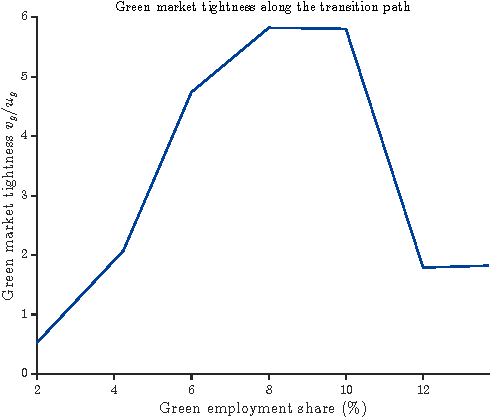
\includegraphics[width=\linewidth]{figure8a.pdf}
    \caption{Green market tightness, $\theta_g \equiv v_g/u_g$, along the welfare-maximizing path. Tightness initially rises as vacancies outpace entrants, peaks when the market becomes very tight, and then declines as policy tilts back toward worker entry.}
    \label{fig:app_transition_tightness}
  \end{subfigure}\hfill
  \begin{subfigure}{0.49\textwidth}
    \centering
    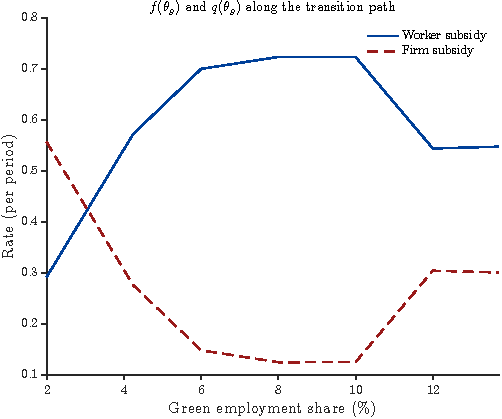
\includegraphics[width=\linewidth]{figure8b.pdf}
    \caption{Job-finding $f(\theta_g)=\text{match}_g/u_g$ and vacancy-filling $q(\theta_g)=\text{mat ch}_g/v_g$ along the same path. As $\theta_g$ rises, $f(\theta_g)$ increases and then flattens mechanically, while $q(\theta_g)$ declines and reaches a trough; when $\theta_g$ later falls, $q(\theta_g)$ recovers.}
    \label{fig:app_transition_rates}
  \end{subfigure}
  \caption{Green labor market dynamics along the transition path.}
  \label{fig:app_transition_tightness_rates}
\end{figure}

% ================= Figure 3 =================
\begin{figure}[H]
  \centering
  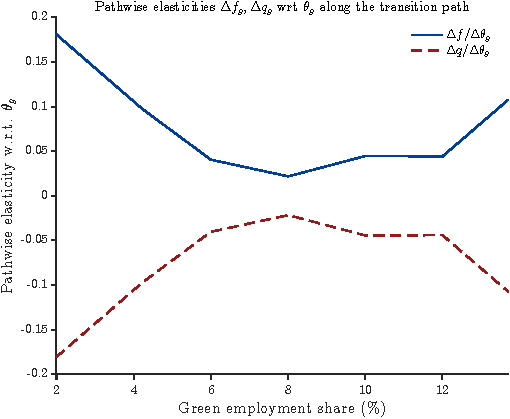
\includegraphics[width=0.6\linewidth]{figure9.pdf}
  \caption{Pathwise sensitivities of matching rates to tightness. Early in the path, $f$ is most responsive to changes in $\theta_g$ while $q$ remains relatively high; mid-path both margins are locally inelastic (low $\partial f/\partial\theta_g$ and $|\partial q/\partial\theta_g|$), and late in the path $q$ becomes more responsive as $\theta_g$ recedes.}
  \label{fig:app_transition_derivatives}
  \vspace{0.5em}
  \begin{minipage}{\linewidth}
    \footnotesize
    \textit{Notes:} Sensitivities are computed as finite differences along the welfare-maximizing sequence of steady states: 
    $\Delta f/\Delta\theta_g$ and $\Delta q/\Delta\theta_g$.
  \end{minipage}
\end{figure}
\end{document}
